% !TEX program = xelatex
% !BIB program = biber
%
% Магистерская НИР — основной файл
% ТвГУ, 2026.  Антонов М.Д.
%
% Сборка: latexmk -xelatex main.tex
% Или:   xelatex main && biber main && xelatex main && xelatex main

\documentclass[14pt,a4paper,oneside]{extarticle}

% --- Geometry (ГОСТ Р 7.0.11-2011) -----------------------------------------
\usepackage[
  left=30mm, right=15mm, top=20mm, bottom=20mm,
  headheight=14pt, footskip=10mm
]{geometry}

% --- Fonts ------------------------------------------------------------------
\usepackage{fontspec}
\setmainfont{Times New Roman}
\setsansfont{Arial}
\setmonofont{Consolas}[Scale=0.92]

% --- Languages --------------------------------------------------------------
\usepackage{polyglossia}
\setdefaultlanguage{russian}
\setotherlanguage{english}

% --- Spacing ----------------------------------------------------------------
\usepackage{setspace}
\onehalfspacing                       % 1.5 line spacing (ГОСТ)
\usepackage{indentfirst}              % indent first paragraph of each section
\setlength{\parindent}{1.25cm}        % 1.25cm красная строка
\setlength{\parskip}{0pt}

% --- Math, symbols ----------------------------------------------------------
\usepackage{amsmath, amssymb, amsthm, mathtools}

% --- Section headings -------------------------------------------------------
\usepackage{titlesec}

% Section becomes "Глава N." prefix (only in main matter, not appendix).
\titleformat{\section}
  {\bfseries\fontsize{14}{16}\selectfont\centering}
  {Глава \thesection.}{0.5em}{}
\titleformat{\subsection}
  {\bfseries\fontsize{13}{15}\selectfont}
  {\thesubsection}{0.7em}{}
\titleformat{\subsubsection}
  {\itshape\fontsize{12}{14}\selectfont}
  {\thesubsubsection}{0.7em}{}

\titlespacing*{\section}{0pt}{18pt}{10pt}
\titlespacing*{\subsection}{0pt}{10pt}{6pt}
\titlespacing*{\subsubsection}{0pt}{8pt}{4pt}

% Appendix uses "Приложение X." instead of "Глава N."
\newcommand{\appendixformat}{%
  \titleformat{\section}
    {\bfseries\fontsize{14}{16}\selectfont\centering}
    {Приложение \thesection.}{0.5em}{}
}

% --- Tables -----------------------------------------------------------------
\usepackage{booktabs}
\usepackage{longtable}
\usepackage{tabularx}
\usepackage{array}
\usepackage{makecell}
\renewcommand{\arraystretch}{1.15}
\newcolumntype{L}[1]{>{\raggedright\arraybackslash}p{#1}}
\newcolumntype{C}[1]{>{\centering\arraybackslash}p{#1}}
\newcolumntype{R}[1]{>{\raggedleft\arraybackslash}p{#1}}

% --- Captions ---------------------------------------------------------------
\usepackage[font=small,labelfont=bf]{caption}

% --- Graphics ---------------------------------------------------------------
\usepackage{graphicx}
\usepackage{float}
\graphicspath{{figures/}{../results/plots/}}

% --- Code listings ----------------------------------------------------------
\usepackage{xcolor}
\usepackage{listings}

% Define languages not bundled with `listings`: JavaScript/TypeScript and bash
\lstdefinelanguage{JavaScript}{
  keywords={break,case,catch,continue,debugger,default,delete,do,else,false,
    finally,for,function,if,in,instanceof,new,null,return,switch,this,throw,
    true,try,typeof,var,void,while,with,let,const,async,await,of,import,export,
    from,class,extends,super},
  ndkeywords={true,false,null,undefined,NaN,Infinity},
  morecomment=[l]{//},
  morecomment=[s]{/*}{*/},
  morestring=[b]',
  morestring=[b]",
  morestring=[b]`,
  sensitive=true
}
\lstdefinelanguage{TypeScript}[]{JavaScript}{
  morekeywords={interface,type,enum,implements,readonly,public,private,protected,
    abstract,as,namespace,declare,module,never,unknown,any,number,string,boolean,
    object,Symbol,bigint},
  sensitive=true
}
\lstdefinelanguage{bash}{
  morekeywords={if,then,else,elif,fi,for,while,do,done,case,esac,return,in,
    function,select,until,export,local,readonly,source,alias,unalias,echo,
    cd,pwd,ls,cat,grep,sed,awk,find,xargs,test},
  morecomment=[l]\#,
  morestring=[b]',
  morestring=[b]",
  sensitive=true
}

\lstset{
  basicstyle=\ttfamily\small,
  keywordstyle=\bfseries\color{blue!60!black},
  commentstyle=\color{gray!70},
  stringstyle=\color{green!50!black},
  breaklines=true,
  frame=single,
  framesep=4pt,
  rulecolor=\color{gray!40},
  numbers=none,
  showstringspaces=false,
  extendedchars=true,
  inputencoding=utf8,
}

% --- Hyperlinks -------------------------------------------------------------
\usepackage[
  bookmarks=true,
  bookmarksopen=true,
  bookmarksnumbered=true,
  unicode=true,
  colorlinks=true,
  linkcolor=black,
  citecolor=black,
  urlcolor=blue!60!black,
  pdfborder={0 0 0}
]{hyperref}

% --- Bibliography -----------------------------------------------------------
\usepackage[
  backend=biber,
  style=gost-numeric,
  language=auto,
  sorting=none,
  maxnames=5,
  giveninits=true
]{biblatex}
\addbibresource{references.bib}

% --- Custom commands --------------------------------------------------------
\newcommand{\code}[1]{\texttt{#1}}
\newcommand{\eg}{например}
\newcommand{\ie}{т.\,е.}

% =============================================================================
\begin{document}

% --- Титульный лист ---------------------------------------------------------
% Титульный лист
\begin{titlepage}
\begin{center}

{\fontsize{12}{14}\selectfont
МИНИСТЕРСТВО НАУКИ И ВЫСШЕГО ОБРАЗОВАНИЯ\\
РОССИЙСКОЙ ФЕДЕРАЦИИ\\[6pt]
ФГБОУ ВО <<Тверской государственный университет>>\\[6pt]
Факультет прикладной математики и кибернетики\\
Кафедра информационных технологий
}

\vspace{4cm}

{\fontsize{16}{20}\selectfont\bfseries
ОТЧЁТ\\
о научно-исследовательской работе
}

\vspace{1.5cm}

{\fontsize{14}{18}\selectfont\itshape
Тема:
}

\vspace{0.5cm}

{\fontsize{15}{19}\selectfont\bfseries
Модуль автоматического анализа\\
музыкальных композиций на основе\\
мульти-задачного глубокого обучения
}

\vfill

\begin{flushright}
\begin{minipage}{0.55\textwidth}
\fontsize{13}{17}\selectfont
\textbf{Выполнил:}\\
магистрант 2 курса\\
Антонов М.\,Д.\\[18pt]

\textbf{Научный руководитель:}\\
доцент кафедры ИТ\\
Кудряшов М.\,Ю.
\end{minipage}
\end{flushright}

\vfill

{\fontsize{12}{14}\selectfont
Тверь, 2026
}

\end{center}
\end{titlepage}
\newpage


% --- Оглавление -------------------------------------------------------------
\tableofcontents
\newpage

% --- Введение ---------------------------------------------------------------
% ============================================================================
%  ВВЕДЕНИЕ
% ============================================================================

\introduction

% ---------------------------------------------------------------------------
\actuality

Промышленные музыкальные сервисы сегодня оперируют каталогами, в которые ежедневно добавляются десятки тысяч новых треков. Только Spotify к 2024 году преодолел отметку в 100 миллионов композиций. Темпы роста каталогов давно превысили физические возможности ручной разметки. В таких условиях возрастает спрос на автоматические инструменты семантической разметки аудио: определение жанра, оценка эмоционального содержания, выделение структурных секций. На рынке такие задачи в большинстве случаев решаются специализированными моделями, каждая под свою задачу, что приводит к избыточному дублированию параметров и не использует общую акустическую природу входных данных. Настоящая работа направлена на проверку гипотезы о том, что объединение четырёх задач (структурной сегментации, классификации возбуждения, валентности и жанра) в единой мультизадачной модели с общим энкодером и независимыми головами не приводит к существенной деградации качества по сравнению с однозадачными моделями, и при этом даёт согласованную разметку за один проход.

% ---------------------------------------------------------------------------
\review

Предметная область опирается на обзорные работы по MIR~\cite{downie2003mir} и применению глубокого обучения~\cite{choi2017tutorial}, на исследования по структурной сегментации (метод матриц автоподобия, глубокие модели, датасет Harmonix~Set), распознаванию эмоций (модель Расселла, датасет DEAM) и жанровой классификации (бенчмарк GTZAN, набор моделей PANNs~\cite{kong2020panns} и архитектура AST~\cite{gong2021ast}). Эти источники служат для формирования гипотез и обоснования сравниваемых архитектур. Полный обзор приведён в Главе~1.

% ---------------------------------------------------------------------------
\goalandtasks

% ---------------------------------------------------------------------------
\tools

Работа опирается на стандартные для области методы цифровой обработки сигналов (короткое преобразование Фурье, лог-мел-спектрограмма, chroma), машинного обучения (свёрточные сети с SE-блоками, двунаправленные LSTM, самовнимание AST с трансфером весов AudioSet), регуляризации (SpecAugment, focal loss, label smoothing, MixUp) и динамического программирования (декодер Витерби с позиционными приорами). Реализация выполнена на Python 3.12 с PyTorch, librosa и scikit-learn. Веб-прототип построен на React 19 с Vite на фронтенде, на Elysia с Bun на бэкенде и на FastAPI с PyTorch на стороне инференса. Полноэкранный визуализатор Vibe Mode использует WebGL2.

% ---------------------------------------------------------------------------
\results

% ---------------------------------------------------------------------------
\originality

Научная новизна работы заключается в следующем. Разработана мультизадачная нейросетевая модель с единым аудио-энкодером и четырьмя классификационными головами, обучаемая одновременно на трёх разнородных датасетах (DEAM, Harmonix Set, GTZAN) по схеме round-robin. Впервые, насколько известно автору, выполнено систематическое сравнение применимости пяти конфигураций (CNN per-window, CNN с надстройкой BiLSTM, PANNs с линейными головами, PANNs с BiLSTM, Audio Spectrogram Transformer с частичной разморозкой) к этой задаче в едином экспериментальном протоколе. Предложен воспроизводимый пайплайн кросс-датасетного обучения через RoundRobinLoader с покомпонентным взвешиванием потерь, в том числе для случая, когда метки каждой задачи присутствуют только в одном из источников. Дополнительно предложен и количественно оценен составной постобработчик сегментных предсказаний (декодер Витерби с матрицей переходов, позиционными приорами и поклассовыми ограничениями минимальной длительности), повышающий Boundary~F1 на 14 пунктов относительно базового аргмакса и сокращающий среднее число выдаваемых сегментов с 28 до 7-8. Также реализован интерактивный веб-прототип с шестипанельным синхронизированным дашбордом и WebGL2-визуализатором, обеспечивающий академически честную коммуникацию ограничений модели (топ-3 жанров с предупреждением об уверенности при out-of-distribution).

% ---------------------------------------------------------------------------
\approbation

Результаты исследования прошли апробацию на студенческой научной конференции факультета прикладной математики и кибернетики Тверского государственного университета (2026 год). По теме работы принята к публикации статья «Мультизадачный анализ музыкальных композиций с помощью предобученного аудио-трансформера» в сборнике трудов конференции. В статью включены лучшие по каждой задаче результаты среди исследованных конфигураций. Помимо этого, разработанный прототип был отдельно протестирован на наборе из 41 аудиотрека различных жанров. Для каждого модель сформировала структурную разметку, эмоциональные кривые и распределение жанров. Реализация оформлена в виде открытого репозитория с 128 автоматическими тестами, обеспечивающими воспроизводимость экспериментов.

% ---------------------------------------------------------------------------
\structure

Работа состоит из введения, семи глав основной части, заключения, списка использованных источников и пяти приложений.

Глава~1 содержит обзор предметной области. В ней разбираются три основные задачи MIR из числа решаемых в работе (структурная сегментация, распознавание эмоций, жанровая классификация), эталонные датасеты по каждой задаче и пять архитектурных семейств для аудио-классификации: свёрточные сети с блоками канального внимания, надстройки двунаправленной LSTM, замороженные эмбеддинги PANNs CNN14 и Audio Spectrogram Transformer с трансфером с AudioSet. Отдельные параграфы посвящены мультизадачному обучению и техникам аккуратного дообучения предобученных моделей.

Глава~2 содержит формальную постановку задачи. Цель работы и четыре класса выходных предсказаний модели формализованы математически: входной аудиосигнал, последовательность лог-мел окон, четыре распределения вероятностей и постобработка во временные интервалы. На основе этой формализации сформулированы пять исследовательских вопросов RQ1--RQ5, легших в основу экспериментальной программы. Завершает главу содержательное обоснование выбора мультизадачного подхода по трём линиям: семантической, методологической и практической.

Глава~3 описывает данные. Подробно разбираются три открытых датасета (DEAM, Harmonix Set, GTZAN), включая их объёмы, лицензии и процедуру скачивания недостающего аудио для Harmonix через \texttt{yt-dlp}. Описан унифицированный пайплайн извлечения логарифмических мел-спектрограмм, окновая нарезка с шагом одна секунда, глобальная нормализация по обучающему сплиту и стратегия разбиения на обучающую, валидационную и тестовую выборки на уровне треков. Отдельный раздел посвящён компенсации сильного дисбаланса классов в структурной задаче через сочетание focal loss, весов классов с верхним порогом и поканальных весов потери.

Глава~4 содержит описание методов. Подробно разобраны все пять архитектурных конфигураций (CNN, CNN+BiLSTM, PANNs+Linear, PANNs+BiLSTM, AST~v2), общая схема мультизадачных голов и функция потерь на основе focal loss, оптимизатор AdamW с расписанием CosineAnnealingWarmRestarts. Отдельный большой раздел разбирает постобработку сегментных предсказаний на основе декодера Витерби: матрица переходов, позиционные приоры, поклассовые ограничения минимальной длительности, расширенная версия v2 с шестью механизмами. Завершает главу описание пайплайна инференса на пользовательских записях.

Глава~5 представляет результаты экспериментов. Описаны протокол оценки и гиперпараметры обучения, после чего излагаются четыре последовательных эксперимента: базовый запуск v1, улучшенный v2, расширение трансформер-архитектурой AST~v2 и неудачный CNN~v3. Сводное сравнение всех конфигураций даётся в отдельном разделе вместе с ablation-экспериментом по компонентам постобработки.

Глава~6 описывает реализованный веб-прототип. Разобрана трёхзвенная архитектура (фронтенд, бэкенд, сервис инференса), синхронизированный дашборд из шести панелей, ключевые UX-решения для честной коммуникации ограничений модели и технологический стек. Завершает главу описание визуального редизайна в стилистике glassmorphism и полноэкранного визуализатора Vibe Mode на WebGL2-шейдере.

Глава~7 содержит сводный анализ результатов. Даны ответы на все пять исследовательских вопросов, зафиксирована финальная конфигурация прототипа, систематически проанализированы пять групп ограничений подхода с возможными направлениями развития, проведено сопоставление со state-of-the-art по каждой задаче, сформулирована научная новизна и практическая значимость работы.

Заключение кратко перечисляет основные результаты и направления дальнейшей работы. Список использованных источников содержит 40 наименований. Пять приложений (А--Д) собирают подробные технические сведения: характеристики датасетов, гиперпараметры конфигураций, путеводитель по графическим результатам, JSON-схему выхода модели и команды воспроизведения экспериментов.


% --- Главы ------------------------------------------------------------------
\section{Обзор предметной области}\label{ch:1}

\subsection{Music Information Retrieval как научная дисциплина}\label{sec:1-1}

\textbf{Music Information Retrieval (MIR)} — междисциплинарная область, объединяющая методы обработки сигналов, машинного обучения, музыкальной теории и психоакустики для извлечения семантической информации из аудиозаписей музыки. Сформировалась как самостоятельное направление в начале 2000-х годов с учреждением ежегодной конференции ISMIR (International Society for Music Information Retrieval) в 2000 году~\cite{downie2003mir}.

Типичные задачи MIR делятся на несколько групп:

\textbf{Классификация на уровне трека} — модель присваивает целому аудиофайлу одну или несколько меток. Сюда относятся определение жанра (genre classification), исполнителя (artist identification), настроения (mood detection), языка вокала. Эти задачи близки к задачам компьютерного зрения image classification.

\textbf{Покадровая разметка (frame-level labeling)} — модель формирует временной ряд предсказаний с заданным шагом. Примеры: транскрипция нот (note onset detection), оценка темпа (tempo tracking), определение тональности (key estimation), извлечение хора (chord recognition).

\textbf{Сегментация (segmentation)} — модель разбивает трек на непрерывные интервалы по структурному, эмоциональному или акустическому признаку. К этой группе принадлежат задачи структурного анализа (Music Structure Analysis), сегментации по эмоциям (emotion segmentation), детекции тишины и переходов.

\textbf{Регрессия на непрерывных шкалах} — оценка непрерывных величин: arousal/valence (по шкалам Russell), tempo BPM, loudness LUFS.

\textbf{Generative задачи} — синтез музыки, генерация аккомпанемента, source separation. В рамках настоящей работы не рассматриваются.

Настоящая работа фокусируется на трёх задачах второй группы (покадровая разметка) и одной задаче первой группы (классификация жанра), решаемых одновременно средствами мульти-задачной модели. Такая постановка отражает практическую потребность создания \textbf{полной семантической разметки} аудиотрека для пользовательских приложений: автоматического создания превью, ритм-игр, музыкальных рекомендательных систем.

\subsubsection{Признаковое представление аудио}

Базовым представлением для MIR-моделей с 2010-х годов является \textbf{мел-спектрограмма} — двумерное представление частотно-временной структуры сигнала, где частотная ось преобразована из линейного герцевого масштаба в перцептивно равномерную мел-шкалу~\cite{stevens1937mel}. Для последующего применения свёрточных сетей логарифмическая компрессия амплитуды (\code{librosa.power\_to\_db}) дополнительно сглаживает динамический диапазон. Получаемое представление (log-mel) сравнимо по информативности с человеческим восприятием тембра и достаточно для большинства классификационных задач.

В данной работе используется log-mel с параметрами: 128 мел-полос (диапазон 30–11025\,Гц при sample rate 22050\,Гц), окно STFT 2048 семплов, hop 512 семплов ($\approx 23$\,мс). Эти значения соответствуют общепринятым практикам в литературе~\cite{choi2017tutorial,kong2020panns}.

Альтернативные представления — chroma (12-полосная гистограмма по нотам), MFCC (мел-кепстральные коэффициенты), constant-Q спектрограмма (CQT) — рассматривались на этапе ablation, но не вошли в финальную модель: вклад chroma в качество классификации оказался несущественным ($\leq 1$\,п.п. accuracy), а вычислительные затраты на CQT при сравнимом качестве не оправданы.

\subsection{Структурная сегментация музыкальных композиций}\label{sec:1-2}

Задача структурной сегментации (Music Structure Analysis, MSA) состоит в автоматическом разбиении аудиотрека на смысловые фрагменты, соответствующие музыкальной форме: вступление (Intro), куплет (Verse), припев (Chorus), бридж (Bridge), инструментальная часть (Instrumental), завершение (Outro). Задача решается на двух уровнях:

\begin{enumerate}
  \item \textbf{Boundary detection} — обнаружение моментов структурных переходов без присвоения меток.
  \item \textbf{Section labeling} — классификация выделенных интервалов в одну из заранее определённых категорий.
\end{enumerate}

Совмещение обеих подзадач в единой модели остаётся открытой проблемой: 6-классовая section labeling считается одной из наиболее сложных задач MIR, поскольку различия между Verse и Chorus определяются не только спектральными признаками, но и контекстом всей композиции (повторяемостью, динамикой, аранжировкой).

\subsubsection{Классические подходы}

До эпохи глубокого обучения структурная сегментация решалась через явное моделирование само-подобия аудио. Ключевая структура — \textbf{self-similarity matrix (SSM)}~\cite{foote2000novelty}, где элемент \code{(i,j)} отражает сходство признаковых векторов в моментах \code{i} и \code{j}. Хор и куплет проявляются как яркие диагональные блоки на SSM, бриджи — как уникальные области без повторов.

На основе SSM строятся:

\begin{itemize}
  \item \textbf{Novelty curve} (Foote, 2000)~\cite{foote2000novelty} — функция, измеряющая локальный контраст SSM по диагонали; пики novelty curve соответствуют границам сегментов.
  \item \textbf{Convex hull algorithm} (Serrà, 2014)~\cite{serra2014unsupervised} — сегментация SSM через выпуклую оболочку диагональных проекций.
  \item \textbf{Spectral clustering на SSM} (McFee \& Ellis, 2014)~\cite{mcfee2014spectral} — группировка похожих временных интервалов через лапласиан матрицы.
\end{itemize}

Достоинства классических методов: интерпретируемость, отсутствие необходимости в большом обучающем наборе, хорошее качество boundary detection (F1 до 0.6–0.7 на SALAMI). Недостатки: требуют тщательной настройки гиперпараметров под конкретный жанр, плохо обобщаются на сложные структуры (электронная музыка с пост-роковыми элементами), не решают section labeling без дополнительного классификатора.

\subsubsection{Подходы на основе глубокого обучения}

С 2014 года доминирующим направлением становятся свёрточные нейронные сети, обучаемые непосредственно на размеченных датасетах:

\begin{itemize}
  \item \textbf{Ullrich et al., 2014}~\cite{ullrich2014boundary} — первая публикация о применении CNN к MSA. Авторы обучают модель предсказывать boundary indicator function (вероятность того, что данный фрейм является границей) на датасете SALAMI. Достигают F1 $\approx 0.46$ при допуске $\pm 3$ секунды — превосходит классические методы.
  \item \textbf{Serrà et al., 2018}~\cite{serra2018cnnhmm} — комбинирует CNN-предсказания с пост-обработкой через HMM с переходными вероятностями. Показывает, что temporal smoothing критичен для устранения «шума» CNN-предсказаний.
  \item \textbf{Wang et al., 2022}~\cite{wang2022catchchorus} — Transformer-based архитектура с self-attention над CNN-эмбеддингами. Достигает F1 $\approx 0.55$ на SALAMI.
  \item \textbf{Gong \& Glass, 2023}~\cite{gong2023structural} — pure-attention модель на основе AST (см. §1.5.5), достигает F1 $\approx 0.62$ на Harmonix.
\end{itemize}

\subsubsection{Ограничения существующих подходов}

Несмотря на прогресс, MSA остаётся самой слабой задачей в ряду MIR-проблем. Типичные значения accuracy section labeling на 6 классах не превышают 40–45\%~\cite{wang2022catchchorus,gong2023structural}. Основные причины:

\begin{enumerate}
  \item \textbf{Class imbalance}: Verse и Chorus составляют 60–70\% размеченного времени в датасетах вроде Harmonix; редкие классы (Outro, Instrumental) — менее 5\%.
  \item \textbf{Inter-annotator disagreement}: даже профессиональные музыканты расходятся в маркировке границ примерно в 15\% случаев, в категории section — в 25\% случаев~\cite{smith2011salami}.
  \item \textbf{Acoustic similarity}: Intro и Outro акустически идентичны (разреженная фактура, сниженная динамика); их можно различить только по позиции в треке. Verse и Pre-chorus также часто неразличимы спектрально.
  \item \textbf{Domain shift}: модели, обученные на классической поп-музыке (Harmonix), плохо обобщаются на электронную, экспериментальную, фолк-музыку.
\end{enumerate}

Современные решения включают пост-обработку через HMM или Viterbi-декодирование с musicological priors~\cite{serra2018cnnhmm,gong2023structural}, что и применяется в настоящей работе (см. §4.7).

\subsection{Распознавание эмоций в музыке}\label{sec:1-3}

Задача Music Emotion Recognition (MER) состоит в автоматической оценке эмоциональной окраски аудиофрагмента. Существуют два основных подхода к формализации:

\subsubsection{Дискретные категории (categorical model)}

В этом подходе каждому фрагменту присваивается одна из заранее определённых эмоциональных меток: «happy», «sad», «aggressive», «calm». Корни подхода восходят к работам Hevner~\cite{hevner1936expression}, предложившей восьмисекторную схему музыкальных аффектов. Современные датасеты (DEAP, MoodSwings) используют 4–8 базовых категорий.

Достоинства: интерпретируемость, прямая совместимость с user interface (emoji-теги). Недостатки: эмоциональное пространство дискретизируется субъективно, теряется тонкая градация.

\subsubsection{Непрерывные шкалы — Russell circumplex model}

Альтернатива — двумерное непрерывное пространство по Russell~\cite{russell1980circumplex}:

\begin{itemize}
  \item \textbf{Valence} — ось «приятное/неприятное» (по горизонтали, $x \in [-1, +1]$).
  \item \textbf{Arousal} — ось «активное/спокойное» (по вертикали, $y \in [-1, +1]$).
\end{itemize}

Russell показал, что большинство эмоциональных оценок музыки можно представить точкой в этом квадранте. Четыре квадранта получают семантические интерпретации:

\begin{table}[H]
\centering
\caption{Семантика квадрантов Russell circumplex}
\begin{tabular}{llll}
\toprule
Квадрант & Valence & Arousal & Семантика \\
\midrule
Q1 & + & + & Радостное (joyful, exhilarating) \\
Q2 & − & + & Злое, тревожное (angry, anxious) \\
Q3 & − & − & Грустное (sad, melancholic) \\
Q4 & + & − & Умиротворённое (peaceful, calm) \\
\bottomrule
\end{tabular}
\end{table}

DEAM dataset~\cite{aljanaki2017deam} предоставляет покадровые непрерывные аннотации arousal/valence для 1802 30-секундных фрагментов. Соглашение между аннотаторами (inter-annotator agreement) измеряется Pearson correlation и составляет $\rho \approx 0.55$–$0.65$ — что считается удовлетворительным для субъективной задачи такого рода.

\subsubsection{Дискретизация в категории}

Несмотря на привлекательность непрерывного подхода, для задач визуализации и пользовательского интерфейса дискретные категории информативнее. В настоящей работе непрерывные оценки DEAM квантизованы в 3 уровня по каждой оси (Low/Mid/High для arousal, Dark/Neutral/Bright для valence), что:

\begin{enumerate}
  \item Снижает вариативность аннотаций (3 категории менее зависимы от субъективных порогов, чем непрерывная шкала).
  \item Упрощает временную сегментацию (3-классовая argmax легко поддаётся median filter).
  \item Сохраняет основную семантическую информацию (низкий/средний/высокий уровень).
\end{enumerate}

При этом исходные непрерывные значения сохраняются как regression targets для дополнительной 2D-визуализации (Russell circumplex в прототипе системы — см. §6.2).

\subsubsection{Подходы к решению}

Для MER применяются те же архитектуры, что и для классификации — CNN (Choi et al., 2017~\cite{choi2017crnn}), CRNN с BiLSTM (Wang et al., 2017~\cite{wang2017autotagging}), Transformer-based (Won et al., 2020~\cite{won2020selfattention}). Текущий SOTA на DEAM 3-классовой arousal: 65–70\% accuracy, valence: 55–60\%. Разрыв между arousal и valence объясняется тем, что arousal сильнее коррелирует со спектральными признаками (громкость, темп, плотность атак), тогда как valence требует понимания мелодико-гармонического контекста, который CNN извлекает менее эффективно.

\subsection{Классификация жанров}\label{sec:1-4}

Genre classification — исторически первая задача MIR, начавшаяся с работы Tzanetakis \& Cook (2002)~\cite{tzanetakis2002gtzan}, которые опубликовали датасет \textbf{GTZAN} — 1000 30-секундных фрагментов в 10 жанрах (blues, classical, country, disco, hip-hop, jazz, metal, pop, reggae, rock).

GTZAN остаётся стандартом сравнения уже более 20 лет, несмотря на известные ограничения~\cite{sturm2014state}:

\begin{itemize}
  \item Дубликаты треков (около 5\% записей повторяются под разными метками).
  \item Ошибки маркировки (особенно в категориях rock/country/blues).
  \item Устаревшая таксономия — не отражает современные жанры (electronic, hip-hop subgenres, indie, lo-fi).
  \item Фрагменты по 30 секунд не передают долгосрочную структуру.
\end{itemize}

Современные альтернативы:

\begin{itemize}
  \item \textbf{FMA (Free Music Archive)}~\cite{defferrard2017fma} — 100 тыс. треков, 161 жанровая категория, multi-label.
  \item \textbf{MagnaTagATune}~\cite{law2009magnatagatune} — 25 тыс. фрагментов с 188 социальными тегами.
  \item \textbf{Million Song Dataset}~\cite{bertinmahieux2011msd} — метаданные 1 млн треков, в том числе пользовательские теги Last.fm.
\end{itemize}

В настоящей работе используется именно GTZAN — несмотря на ограничения — поскольку это позволяет напрямую сопоставить полученные результаты с обширной литературой и сохранить сравнимость с baseline-моделями. \textbf{Ограничения out-of-distribution} (поведение на современных жанрах вне 10 категорий GTZAN) явно адресуются в прототипе системы через UI-механизм top-3 классификаций с предупреждением о низкой уверенности (см. §6.3).

Текущие SOTA-результаты на GTZAN:

\begin{table}[H]
\centering
\caption{SOTA-результаты на GTZAN}
\begin{tabular}{llll}
\toprule
Архитектура & Год & Accuracy & Источник \\
\midrule
MFCC + SVM & 2002 & 61\% & Tzanetakis~\cite{tzanetakis2002gtzan} \\
CNN baseline & 2015 & 75\% & Sigtia~\cite{sigtia2014improved} \\
CRNN & 2017 & 79\% & Choi~\cite{choi2017crnn} \\
Multi-DNN ensemble & 2018 & 82\% & Sturm~\cite{sturm2014state} \\
PANNs (CNN14, AudioSet pretrained) & 2020 & 87\% & Kong~\cite{kong2020panns} \\
AST (Audio Spectrogram Transformer) & 2021 & 89\% & Gong~\cite{gong2021ast} \\
\bottomrule
\end{tabular}
\end{table}

В рамках настоящей работы достигнут показатель 83.9\% (CNN v2, обучение с нуля) и 81.5\% (AST v2, fine-tuned), что соответствует среднему уровню современных решений на GTZAN.

\subsection{Архитектуры аудио-классификаторов}\label{sec:1-5}

\subsubsection{Свёрточные нейронные сети (CNN)}

Свёрточные сети применяются к log-mel спектрограмме как к двумерному «изображению» с одним каналом. Базовый блок состоит из 2D-свёртки 3$\times$3, пакетной нормализации (BatchNorm) и нелинейности ReLU. Последовательность нескольких таких блоков с MaxPool 2$\times$2 формирует backbone, преобразующий спектрограмму в компактный feature vector через global average pooling (GAP).

Преимущества CNN: высокая параметрическая эффективность ($\sim$1M параметров), хорошее качество на однозадачных бенчмарках, быстрое обучение (3–5 часов на GPU). Недостатки: ограниченное receptive field (порядка 5–10 секунд), плохое моделирование долгосрочных зависимостей, отсутствие предобучения на больших корпусах.

В настоящей работе baseline CNN построен из 5 conv-блоков (32 $\to$ 64 $\to$ 128 $\to$ 256 $\to$ 512 каналов) с механизмом Squeeze-and-Excitation после каждого блока. Подробное описание архитектуры — в §4.2.

\subsubsection{Squeeze-and-Excitation (SE)}

Squeeze-and-Excitation~\cite{hu2018se} — механизм channel attention, добавляемый к CNN-блокам. Идея: после каждого conv-слоя вычисляется глобальный средний канал (squeeze), пропускается через две полносвязные операции с sigmoid (excitation), и полученные веса умножаются на исходные каналы. Это позволяет модели динамически усиливать «важные» частотные диапазоны и ослаблять неинформативные.

Эффект SE-блоков на MIR-задачах: улучшение accuracy на 1–3 п.п. при увеличении числа параметров на 5–10\%. В нашей работе SE-блоки добавлены после каждого из 5 conv-блоков.

\subsubsection{BiLSTM для temporal modeling}

Bidirectional LSTM~\cite{hochreiter1997lstm} — рекуррентная сеть, обрабатывающая последовательность в обоих направлениях. В контексте MIR применяется как «голова» поверх CNN-эмбеддингов: трек разбивается на окна, каждое окно сжимается CNN в вектор фиксированной размерности, и LSTM строит контекстуально-зависимое представление каждого окна.

Преимущество BiLSTM перед per-window классификацией: учёт долгосрочного контекста (LSTM «помнит» что было 30+ секунд назад). Недостатки: количество обучающих примеров уменьшается (одна последовательность вместо $\sim$200 окон $\to$ потеря разнообразия), повышенный риск переобучения.

В нашей работе BiLSTM-варианты (CNN+BiLSTM, PANNs+BiLSTM) — часть 2$\times$2 факторного эксперимента; результаты см. §5.4.

\subsubsection{PANNs — pretraining на AudioSet}

\textbf{PANNs (Pretrained Audio Neural Networks)}~\cite{kong2020panns} — семейство CNN-моделей, предобученных на датасете AudioSet ($\sim$2M YouTube-фрагментов, 527 категорий звуков). Наиболее популярная модель — CNN14, выдающая 2048-мерный embedding на каждое 1-секундное окно.

Применение PANNs как «замороженного» feature extractor — стандартный transfer learning paradigm в современном MIR: вместо обучения CNN с нуля используются готовые embedding, и обучается только классификационная голова. Преимущество: сильный inductive bias из AudioSet (миллионы примеров vs наши тысячи). Недостаток: фиксированные представления не адаптируются под специфику задачи.

В настоящей работе PANNs сравнивается с обучаемой с нуля CNN в рамках 2$\times$2 эксперимента (см. §5.3).

\subsubsection{Audio Spectrogram Transformer (AST)}

Наиболее значимый архитектурный прорыв в MIR за последние годы — \textbf{Audio Spectrogram Transformer}~\cite{gong2021ast}, предложенный Gong et al. (2021). AST впервые применил парадигму \textbf{Vision Transformer}~\cite{dosovitskiy2021vit} к аудио-спектрограммам, отказавшись от свёрток в пользу чистого self-attention.

\textbf{Принцип работы:}

\begin{enumerate}
  \item Log-mel спектрограмма размером 128 $\times$ T делится на патчи 16 $\times$ 16 (с перекрытием 6 пикселей по обеим осям).
  \item Каждый патч линейно проецируется в 768-мерный токен.
  \item Добавляются positional embeddings (learnable) и специальный CLS-токен.
  \item Последовательность токенов подаётся на 12-слойный Transformer-encoder с 12 attention heads.
  \item Классификация выполняется по выходу CLS-токена через линейный слой.
\end{enumerate}

Общее число параметров: 87M, из которых $\sim$85M — в трансформере, остальное в эмбеддингах и голове.

\textbf{Pretraining на AudioSet.} Авторы AST предобучают модель на классификации 527 категорий AudioSet через multi-label cross-entropy. Длительность предобучения: $\sim$5 дней на 8 V100 GPU. Готовые веса распространяются под именем \code{MIT/ast-finetuned-audioset-10-10-0.4593} (числа в названии — параметры frequency/time strides и downstream accuracy на AudioSet).

\textbf{Преимущества AST:}

\begin{enumerate}
  \item \textbf{Глобальное восприятие} — self-attention видит каждый патч в контексте всей спектрограммы, что критично для структурного анализа (припев должен «помнить» как звучит куплет).
  \item \textbf{Transfer learning} — pretraining на 2M аудио предоставляет богатые представления, недоступные при обучении с нуля на 2.5K треков.
  \item \textbf{Унифицированная архитектура} — один и тот же модель подходит для всех MIR-задач (segment, emotion, genre).
\end{enumerate}

\textbf{Недостатки:}

\begin{enumerate}
  \item \textbf{Большой checkpoint} — 574\,MB (vs $\sim$21\,MB у CNN).
  \item \textbf{Более медленный inference} — 8 секунд на 3-минутный трек (vs 2 секунды у CNN) на одном GPU.
  \item \textbf{Чувствительность к гиперпараметрам fine-tuning} — слишком агрессивное размораживание layers ведёт к catastrophic forgetting.
\end{enumerate}

В настоящей работе AST применён как финальная модель прототипа после fine-tuning на DEAM+Harmonix+GTZAN с замораживанием первых 8 из 12 transformer-слоёв. Подробное описание fine-tuning стратегии — в §4.5.

\subsection{Multi-task learning в MIR}\label{sec:1-6}

\textbf{Multi-task learning (MTL)}~\cite{caruana1997mtl} — парадигма обучения, при которой одна модель решает несколько связанных задач одновременно через общий backbone и специализированные «головы» для каждой задачи. Идея: связанные задачи разделяют полезные представления, и совместное обучение действует как форма регуляризации, повышающая обобщающую способность.

В MIR multi-task learning естественно мотивирован тем, что задачи структурного, эмоционального и жанрового анализа взаимосвязаны:

\begin{itemize}
  \item \textbf{Genre влияет на структуру}: рок-композиции имеют чётко выраженную verse-chorus форму, классическая музыка — более свободную (sonata-form, fugue), электронная — секциями build-up/drop.
  \item \textbf{Эмоциональная динамика коррелирует со структурой}: переход куплет $\to$ припев типично сопровождается ростом arousal и сменой valence (pre-chorus как «подготовка» эмоционального пика).
  \item \textbf{Жанр и эмоция связаны}: metal статистически чаще тёмный и активный (Q2 квадрант), classical часто спокойный и позитивный (Q4), blues — спокойный и тёмный (Q3).
\end{itemize}

Эти корреляции делают MTL естественной парадигмой: общий backbone извлекает универсальные акустические признаки, головы адаптируют их под конкретную задачу. Кроме того, MTL действует как регуляризатор — модель вынуждена обучаться представлениям, полезным для всех задач сразу, что снижает переобучение на малых датасетах.

\textbf{Технические подходы к MTL:}

\begin{enumerate}
  \item \textbf{Joint loss optimization} — суммарный loss $L = \sum w_i \cdot L_i$ с фиксированными или адаптивными весами.
  \item \textbf{Round-robin batching} — каждый батч содержит примеры из одного датасета, циклически чередуются; backward выполняется только по доступным головам.
  \item \textbf{Adversarial / gradient surgery} методы (PCGrad, GradNorm) — балансировка градиентов между задачами.
\end{enumerate}

В настоящей работе используется первый и второй подходы: round-robin loader формирует батчи DEAM/Harmonix/GTZAN последовательно, loss суммируется по 4 головам с фиксированными per-task весами (segment: 1.5, остальные: 1.0).

\subsection{Pretraining + fine-tuning paradigm}\label{sec:1-7}

Стратегия «предобучение на большом корпусе $\to$ дообучение на целевой задаче» — доминирующий подход во всех областях глубокого обучения с конца 2010-х. В MIR эта парадигма реализуется через AudioSet-pretrained модели (PANNs, AST).

\textbf{Differential learning rate} — техника, при которой разные части модели получают разные learning rates. Обычно:

\begin{itemize}
  \item Pretrained backbone — низкий LR (1e-5 .. 5e-5), чтобы не «сломать» предобученные представления.
  \item Свежеинициализированные heads — высокий LR (1e-3 .. 1e-4), чтобы быстро обучить task-специфичные классификаторы.
\end{itemize}

\textbf{Layer freezing} — частичная или полная заморозка pretrained слоёв. Полная заморозка превращает модель в feature extractor (PANNs+Linear). Частичная (например, заморозить первые 8 из 12 слоёв трансформера) позволяет верхним слоям адаптироваться к специфике задачи без catastrophic forgetting.

\textbf{Gradient accumulation} — при ограниченной GPU-памяти effective batch size наращивается через накопление градиентов по нескольким микро-батчам перед optimizer step. В нашей работе AST обучается с batch\_size=16, grad\_accumulation=4, что даёт effective batch=64.

Применение этих техник к AST в данной работе позволило за 3 часа обучения превзойти CNN-baseline по segment accuracy на 5.3 п.п. при сравнимом качестве на остальных задачах (см. §5.4).

\textbf{Резюме главы 1.} Анализ литературы показывает: (а) MSA остаётся самой сложной задачей MIR с типичной accuracy 30–45\%; (б) классические методы (SSM, novelty curve) уступают современным CNN/Transformer, но дают интерпретируемые границы; (в) Russell circumplex — общепринятая модель эмоций, дискретизация в 3 класса упрощает задачу без потери семантики; (г) GTZAN — устаревший, но стандартный бенчмарк для жанра; (д) AST с pretraining на AudioSet — текущий SOTA в audio classification, превосходит CNN и PANNs в transfer learning. Все эти выводы определяют архитектурные решения настоящей работы.

\chapter{Постановка задачи}\label{ch:2}

\section{Цель исследования}\label{sec:2-1}

Цель работы~--- создать прототип программно-аналитической системы автоматического анализа музыкальных композиций, которая по входному аудиотреку формирует многоаспектную временную разметку (англ. timeline) сразу по четырём категориям признаков. Структурная сегментация выделяет шесть классов музыкальной формы (Intro, Verse, Bridge, Chorus, Instrumental, Outro). Возбуждение (arousal) представлено тремя категориями уровня энергии (Low, Mid, High). Валентность (valence) аналогично имеет три класса эмоциональной окраски (Dark, Neutral, Bright). Жанр выбирается из десяти стандартных категорий GTZAN: blues, classical, country, disco, hip-hop, jazz, metal, pop, reggae, rock.

В отличие от специализированных решений вроде Madmom, Essentia или MIRtoolbox~\cite{bock2016madmom,bogdanov2013essentia,lartillot2007mirtoolbox}, которые решают каждую задачу отдельной моделью, в данной работе все четыре задачи решаются одной мультизадачной моделью. У такого подхода несколько содержательных преимуществ. Структурные границы вычисляются на тех же признаках, что и эмоциональные переходы, поэтому смена секции и смена эмоции не смещаются друг относительно друга. За один проход модели формируются все четыре разметки сразу, без четырёхкратного перерасчёта эмбеддингов. Наконец, единая модель открывает возможность согласованной интерпретации результатов в прототипе (§6.2).

\subsection{Формальная постановка}

Пусть $x \in \mathbb{R}^{T_{\text{audio}}}$ моноаудиосигнал с частотой дискретизации $sr = 22050$~Гц. Извлечение признаков переводит его в последовательность лог-мел окон $X = \{X_1, \dots, X_N\}$, $X_i \in \mathbb{R}^{F \times W}$, где $F = 128$~--- число мел-фильтров, а $W$~--- число STFT-фреймов в окне длительностью $\tau = 10$~с. Для конфигурации librosa с центрированием окон (\texttt{center=True}) и шагом $h = 512$ число фреймов определяется как
\[
W = 1 + \left\lfloor \frac{sr \cdot \tau}{h} \right\rfloor = 1 + \left\lfloor \frac{22050 \cdot 10}{512} \right\rfloor = 431.
\]
Модель $f_\theta$ выдаёт для каждого окна четыре распределения вероятностей:
\[
f_\theta(X_i) = \big( p^{\text{seg}}_i, \; p^{\text{aro}}_i, \; p^{\text{val}}_i, \; p^{\text{gen}}_i \big),
\]
где $p^{\text{seg}}_i \in \Delta^5$, $p^{\text{aro}}_i, p^{\text{val}}_i \in \Delta^2$, $p^{\text{gen}}_i \in \Delta^9$. Здесь $\Delta^{k} = \{\, y \in \mathbb{R}^{k+1}_{+} : \sum_j y_j = 1 \,\}$~--- стандартный $k$-мерный вероятностный симплекс, то есть распределение по $k+1$ классам. Соответственно $\Delta^5$ задаёт распределение по 6 классам сегментации, $\Delta^2$~--- по 3 классам возбуждения и валентности, $\Delta^9$~--- по 10 жанрам. Постобработка $g$ далее преобразует покадровые предсказания в непрерывные интервалы:
\[
g\big( \{p_i\}_{i=1}^N \big) \mapsto \{ (t_j^{\text{start}}, t_j^{\text{end}}, c_j, \kappa_j) \}_{j=1}^M,
\]
где $c_j$~--- класс сегмента, $\kappa_j$~--- степень уверенности модели, $M$~--- итоговое число сегментов после слияния. Конкретная реализация $g$ (декодирование Витерби с позиционными априорными распределениями и слиянием коротких сегментов по минимальной длительности) описывается в §4.7.

\section{Исследовательские вопросы}\label{sec:2-2}

Исследование строилось вокруг пяти вопросов.

Прежде всего, исследовалась жизнеспособность самого мультизадачного подхода: насколько эффективна мультизадачная свёрточная сеть для одновременного решения четырёх задач на относительно небольшом объёме данных (около 2{,}5 тысяч треков) и сопоставимо ли её качество с однозадачными моделями из литературы?

Далее изучался вклад двух независимых факторов в качество модели. Один из них это временное моделирование с помощью BiLSTM поверх покадровых эмбеддингов свёрточной сети: насколько такое усложнение архитектуры оправдано, особенно для структурной сегментации, которая по природе своей требует учёта длинного контекста. Другой фактор это качество входных признаков: даёт ли использование предобученных эмбеддингов PANNs CNN14 (обученных на AudioSet) преимущество перед свёрточной сетью, обученной с нуля на тех же целевых данных.

Следующий вопрос обобщал предыдущие и спрашивал, какой из этих двух факторов важнее и являются ли их эффекты аддитивными или интерактивными.

Наконец, отдельный вопрос был сформулирован уже после первых экспериментов: способна ли архитектура AST, тоже предобученная на AudioSet, но устроенная принципиально иначе (трансформер с самовниманием вместо свёрток), превзойти оба ранее рассмотренных семейства? И если да, то на каких именно задачах преимущество максимально?

Первые четыре вопроса формируют классический $2 \times 2$ факторный эксперимент с четырьмя конфигурациями: CNN per-window, CNN+BiLSTM, PANNs+Linear, PANNs+BiLSTM. Последний вопрос расширяет схему пятой архитектурой (AST). Дополнительно в работу включён ablation-эксперимент по постобработке предсказаний (с декодером Витерби и без, с позиционными априорными распределениями и без).

\section{Обоснование мультизадачного подхода}\label{sec:2-3}

Выбор единой мультизадачной модели обусловлен содержательными, методологическими и практическими факторами, каждый из которых сам по себе является достаточным основанием для отказа от схемы из четырёх независимых моделей.

Прежде всего, выбранные задачи в музыке тесно связаны содержательно. Жанр во многом определяет типичную структуру композиции: рок строится из чередования куплета и припева, симфония подчинена сонатной форме, электронная музыка опирается на схему build-up и drop. Эмоциональная динамика обычно согласована со структурой: переход от куплета к припеву чаще всего сопровождается ростом возбуждения и сменой валентности. Жанр коррелирует и с типичной эмоциональной окраской: металл чаще оказывается в квадранте «злобное-активное», классика в «умиротворённое-спокойное», блюз в «грустное-спокойное». Эти связи модели проще выучивать совместно, чем порознь.

Второй довод методологический. Общий ствол сети при мультизадачном обучении вынужден извлекать максимально универсальные признаки (тембр, ритм, гармония), полезные сразу для всех голов. Это работает как регуляризатор и снижает риск переобучения на признаки, специфические для какой-то одной задачи. Полученные метрики качества в целом сопоставимы с диапазоном опубликованных однозадачных результатов для GTZAN, DEAM и Harmonix~Set (см. сопоставление со state-of-the-art в §7.4).

К ним добавляется и чисто практическая сторона дела. Если запускать четыре отдельные модели последовательно на одном треке, время инференса вырастает в четыре раза (порядка 32 секунд против 8 на трёхминутный трек на использованной видеокарте). Четыре независимые модели могут давать и несогласованные предсказания: граница секции от одной модели не совпадает с моментом эмоционального перехода от другой. Развёртывание приходится поддерживать сразу для четырёх чекпоинтов. Единая мультизадачная модель эти проблемы снимает, что особенно важно для интерактивного веб-прототипа (Глава 6).

\chapter{Данные}\label{ch:3}

В работе используются три открытых датасета, каждый из которых исторически специализировался под одну из решаемых задач: DEAM для эмоций, Harmonix Set для структурной разметки и GTZAN для жанровой классификации. Объединение трёх таких разнородных корпусов в общем мультизадачном пайплайне требует унифицированной предобработки и аккуратных сплитов. Оба вопроса разбираются в этой главе.

\section{Используемые датасеты}\label{sec:3-1}

Сводная информация о датасетах приведена в табл.~\ref{tab:datasets}.

\begin{table}[H]
\centering
\caption{Используемые датасеты}
\label{tab:datasets}
\footnotesize
\setlength{\tabcolsep}{4pt}
\begin{tabular}{L{2.3cm}L{2.5cm}L{1.4cm}L{3.2cm}L{1.9cm}L{2.7cm}}
\toprule
Датасет & Размер & Аудио & Аннотации & Задача & Источник \\
\midrule
DEAM & 1802 фрагмента (45~с каждый) & mp3 & Покадровые непрерывные arousal/valence & Эмоции & MediaEval 2013--2018~\cite{aljanaki2017deam} \\
Harmonix Set & 912 треков (полная длительность) & mp3 (загружено 743) & Структурная разметка с временными метками & Сегментация & Nieto и соавт., 2019~\cite{nieto2019harmonix} \\
GTZAN & 999 фрагментов (30~с каждый) & wav & Жанровая метка целиком на трек & Жанр & Tzanetakis \& Cook, 2002~\cite{tzanetakis2002gtzan} \\
Итого & 3713 уникальных файлов & \multicolumn{2}{l}{$\approx 110$~ГБ извлечённых признаков} & 4 задачи & \\
\bottomrule
\end{tabular}
\end{table}

DEAM~\cite{aljanaki2017deam} это один из крупнейших открытых датасетов для распознавания музыкальных эмоций, собранный в рамках конкурсов MediaEval с 2013 по 2018 годы. Корпус включает 1802 фрагмента по 45 секунд из коллекции Free Music Archive (лицензия Creative Commons). Для каждого фрагмента собрана непрерывная покадровая разметка возбуждения и валентности по краудсорсингу: около десяти аннотаторов на трек с шагом 500 миллисекунд. Поставляется он в виде нескольких CSV: усреднённые ряды по 60 фреймам, стандартные отклонения как оценка согласия аннотаторов и общие метаданные. В данной работе непрерывные значения дискретизируются в три категории по порогам $\pm 0.2$: значения ниже $-0.2$ относятся к классу Low (или Dark для валентности), от $-0.2$ до $+0.2$ к классу Mid (Neutral), выше $+0.2$ к High (Bright). Пороги выбирались так, чтобы получить приблизительно равномерное распределение классов (25--40\,\% на класс) и при этом сохранить семантическую осмысленность границ; разбиение по квантилям такой осмысленности не давало.

Harmonix Set~\cite{nieto2019harmonix} это единственный крупный открытый корпус со структурной разметкой коммерческой популярной музыки. Всего в нём 912 треков, для которых вручную в Sonic Visualiser размечены позиции долей, сильных долей и границы секций. На этапе планирования рассматривались также SALAMI и Beatles, но первый смещён в сторону классики и джаза (что плохо согласовалось с двумя другими задачами работы, ориентированными на поп-сцену), а второй слишком мал по объёму. Из всей разметки Harmonix используются только секции. Авторская таксономия включает 17 категорий, что для шестиклассовой постановки избыточно: они сведены к шести базовым меткам. Все вступления (intro, intro\_a, intro\_b) сливаются в Intro; куплеты и темы (verse, verse\_a, verse\_b, theme) в Verse; переходы и переходные секции (bridge, transition, transition\_a) в Bridge; припевы и хуки (chorus, chorus\_a, hook) в Chorus; инструменталы, соло и брейкдауны в Instrumental; концовки и затухания в Outro. Сами аудиозаписи Harmonix Set по понятным причинам не распространяет. Для их скачивания в рамках работы реализован отдельный скрипт (\code{scripts/download\_harmonix\_audio.py}), который по полю \code{youtube\_id} из аннотации загружает аудио через \code{yt-dlp}. Из 912 треков успешно загрузилось 743 (около 81.5\%). Остальные за прошедшие годы удалены с YouTube правообладателями.

GTZAN~\cite{tzanetakis2002gtzan} в работе используется в стандартном виде: 999 рабочих файлов (один оригинальный wav оказался повреждён) разбиты на десять жанров по сто примеров в каждом, длительность одного фрагмента 30 секунд. Жанры стандартные для бенчмарка: blues, classical, country, disco, hip-hop, jazz, metal, pop, reggae, rock. Известные проблемы GTZAN не игнорируются~\cite{sturm2014state}: около 5\,\% файлов представляют собой дубликаты или near-duplicates, у части примеров спорная разметка, есть выраженный artist bias и общая устаревшая таксономия. Несмотря на это, GTZAN сохранён как основной датасет жанровой задачи, поскольку он остаётся единственным практическим способом сопоставимости с двадцатилетней литературой по теме. Поведение модели на современной музыке дополнительно смягчается стратегией top-3 в прототипе (§6.3).

\section{Извлечение признаков}\label{sec:3-2}

Все три датасета унифицируются на этапе извлечения признаков. Из mp3 или wav librosa загружает моноаудио с частотой дискретизации 22050 Гц, после чего считается логарифмическая мел-спектрограмма со стандартными для задач классификации музыки параметрами: 128 мел-фильтров в диапазоне от 30 Гц до частоты Найквиста (11025 Гц), окно STFT в 2048 отсчётов (около 93 миллисекунд) и шаг между фреймами 512 отсчётов (около 23 миллисекунд). Полученные значения мощности логарифмируются через \code{librosa.power\_to\_db(ref=np.max)}, что переводит спектрограмму в шкалу примерно от $-80$ до $0$ децибел.

Полученные спектрограммы сохраняются в файлах формата npz и далее уже не пересчитываются: при каждой эпохе обучения готовые массивы просто читаются с диска. Для скорости это критично. Без такого кэша из-за стоимости декодирования mp3 каждая эпоха стоила бы кратно дороже.

Параметры подытожены в табл.~\ref{tab:logmel-params}.

\begin{table}[H]
\centering
\caption{Параметры логарифмической мел-спектрограммы}
\label{tab:logmel-params}
\begin{tabular}{L{3cm}L{3cm}L{8cm}}
\toprule
Параметр & Значение & Обоснование \\
\midrule
Sample rate & 22050~Гц & Стандарт librosa, покрывает до 11025~Гц \\
\code{n\_fft} & 2048 & STFT окно около 93~мс \\
\code{hop\_length} & 512 & Шаг между фреймами около 23~мс \\
\code{n\_mels} & 128 & Стандарт для классификации музыки \\
\code{fmin} & 30~Гц & Нижняя граница мел-фильтров \\
\code{fmax} & 11025~Гц & Частота Найквиста \\
\bottomrule
\end{tabular}
\end{table}

Затем спектрограмма каждого трека режется на окна одинаковой длительности. В работе используются окна по 10 секунд (431 спектральный фрейм при выбранных параметрах) с шагом 1 секунда между соседними окнами. Длительность 10 секунд выбрана по двум причинам. Первая: этого хватает на типичный музыкальный период (куплет или припев целиком), что критично для структурной задачи. Вторая: AST предобучен ровно на десятисекундных окнах AudioSet, и сохранение этой длительности позволяет использовать предобученные позиционные эмбеддинги без интерполяции. Шаг в одну секунду даёт около пятидесяти окон на минуту записи, чего более чем достаточно для последующего декодирования Витерби.

Сразу после нарезки выполняется глобальная нормализация. По обучающему сплиту вычисляются средние значения и стандартные отклонения отдельно по каждой мел-полосе, сохраняются в \code{stats.npz}, а далее применяются ко всем сплитам: на каждом окне из каждого мел-фильтра вычитается соответствующее среднее и делится на стандартное отклонение. Тот же \code{stats.npz} используется и при инференсе пользовательских аудиозаписей: \code{musicml/infer.py} загружает его автоматически. Без этого шага на инференсе наблюдался характерный сбой: блюзовая запись с высокой долей низких частот ошибочно распознавалась как hip-hop из-за того, что её распределение энергии по фильтрам оказывалось сдвинуто относительно нормализованного обучающего распределения.

\section{Стратегия разбиения на обучающую, валидационную и тестовую выборки}\label{sec:3-3}

Каждый из трёх датасетов разбивается независимо в соотношении 70/15/15 с фиксированным сидом 42. Главное принципиальное решение здесь, ради которого пришлось аккуратно реализовать сплитер, состоит в том, что разбиение делается на уровне треков, а не на уровне окон. Если резать окна и распределять их случайно, окна одного и того же трека неизбежно попадают и в обучающую, и в тестовую выборки, что искусственно завышает метрики обобщения.

Для GTZAN стратификация по жанрам делается автоматически (по сто треков на каждый из десяти классов). Для DEAM стратификация по эмоциональным классам невозможна в принципе: метки покадровые и непрерывные, а разные фрагменты одного трека вполне могут оказаться в разных классах после квантизации, поэтому используется случайное разбиение. Harmonix тоже разбивается случайно: жанровая информация в нём отсутствует, а стратифицировать по структуре бессмысленно, поскольку все треки покрывают все секции. Списки треков каждого сплита сохраняются в \code{splits.json} для воспроизводимости любого запуска.

\section{Дисбаланс классов}\label{sec:3-4}

Из четырёх рассматриваемых задач три (возбуждение, валентность, жанр) сбалансированы практически по построению или близки к этому, и для них специальной обработки не требуется. Иначе обстоит дело со структурной сегментацией, где классы распределены сильно неравномерно: куплет и припев в сумме занимают около 60\% общего времени обучающих треков, тогда как на концовку приходится меньше 10\%. Распределение классов сведено в табл.~\ref{tab:class-distribution}.

\begin{table}[H]
\centering
\caption{Распределение классов в обучающих сплитах}
\label{tab:class-distribution}
\begin{tabular}{L{3cm}L{3cm}L{3cm}L{4cm}}
\toprule
Задача & Класс & Доля окон & Вес inverse-frequency \\
\midrule
Segment & Verse & $\sim$35\% & 0.71 \\
 & Chorus & $\sim$25\% & 1.00 \\
 & Bridge & $\sim$12\% & 2.08 \\
 & Intro & $\sim$10\% & 2.50 (обрезан) \\
 & Instrumental & $\sim$10\% & 2.50 (обрезан) \\
 & Outro & $\sim$8\% & 2.50 (обрезан) \\
Arousal & Low / Mid / High & $\sim$33\% / 34\% / 33\% & $\approx 1.00$ каждый \\
Valence & Dark / Neutral / Bright & $\sim$33\% / 33\% / 34\% & $\approx 1.00$ каждый \\
Genre & любой из 10 жанров & $\sim$10\% каждый & $\approx 1.00$ каждый \\
\bottomrule
\end{tabular}
\end{table}

Без специальной обработки дисбаланса модель склонна к вырожденному решению с преимущественным предсказанием доминирующих классов. Чтобы этого избежать, в работе применяются сразу три механизма, действующие на разных уровнях. На уровне функции потерь применяется focal loss~\cite{lin2017focal} с показателем $\gamma = 1.5$: множитель $(1 - p_t)^\gamma$ уменьшает вклад тех примеров, по которым модель уже уверена и обычно права, перенаправляя градиент на трудные случаи. На уровне отдельных классов используются веса, обратно пропорциональные частотам, но с верхним порогом 2.5. Без такого порога редкие классы получали бы слишком большой вес и провоцировали обратную проблему. Наконец, на уровне общей мультизадачной потери головам сегментации присваивается дополнительный вес 1.5, тогда как остальным задачам по 1.0.

Эмпирически эти три ограничения находятся в довольно узком оптимуме. В одном из экспериментов (CNN v3, см. §5.5) была проверена гипотеза об одновременном усилении всех трёх механизмов: вес головы сегментации до 3.5, $\gamma$ до 2.5, верхний порог весов классов до 3.5. Модель в результате переобучилась на редкие классы и потеряла около 13 процентных пунктов на сегментной задаче. Эта неудача стала одним из главных аргументов в пользу того, что в задаче компенсации дисбаланса дальнейшее усиление веса редких классов приводит к обратному переобучению.

\section{Архитектура и методы}\label{ch:4}

В работе исследуется пять архитектурных конфигураций, отражающих три измерения дизайна: \textbf{способ извлечения признаков} (обучаемая с нуля CNN vs предобученная PANNs vs трансформер AST), \textbf{наличие temporal modeling} (per-window vs BiLSTM-последовательность) и \textbf{парадигму трансфера} (обучение с нуля vs fine-tuning). Все пять архитектур выпускают одинаковый интерфейс — четыре независимые классификационные головы и две головы регрессии (arousal/valence continuous), что обеспечивает корректное сравнение качества при едином пост-процессинге. Финальная модель прототипа — Audio Spectrogram Transformer v2 с пост-процессингом через Viterbi-декодирование и musicological position priors.

\subsection{Обзор многоархитектурного эксперимента}\label{sec:4-1}

Сводная характеристика пяти архитектур приведена в таблице 4.1.

\begin{table}[H]
\centering
\caption{Таблица 4.1. Сравнение пяти архитектур}
\begin{tabular}{L{0.5cm}L{2.5cm}L{3cm}L{2.2cm}L{3cm}L{1.8cm}L{2.5cm}}
\toprule
№ & Конфиг & Backbone & Temporal & Pretraining & Параметров & Trainable \\
\midrule
1 & CNN & 5-блочная CNN с SE & per-window & нет & $\sim$800K & $\sim$800K \\
2 & CNN+BiLSTM & CNN→BiLSTM(128) & sequence & нет & $\sim$1.2M & $\sim$1.2M \\
3 & PANNs+Linear & PANNs CNN14 & per-window & AudioSet (frozen) & $\sim$80M & $\sim$210K (heads only) \\
4 & PANNs+BiLSTM & PANNs→Proj→BiLSTM(256) & sequence & AudioSet (frozen) & $\sim$81M & $\sim$750K \\
5 & AST v2 & Vision Transformer & per-window (global attn) & AudioSet (fine-tuned) & $\sim$87M & \textbf{$\sim$14M} (heads + 4 unfrozen layers) \\
\bottomrule
\end{tabular}
\end{table}

Конфигурации 1–4 формируют 2$\times$2 факторный эксперимент, отвечающий на RQ1–RQ4 (см. §2.2). Конфигурация 5 — расширение эксперимента трансформер-парадигмой, отвечает на RQ5 и используется как финальная модель прототипа.

\subsection{CNN backbone (конфигурация 1)}\label{sec:4-2}

\subsubsection{Архитектура}

\begin{lstlisting}
Input: (B, 1, 128, T)   batch x channels x mel_bins x time_frames

Conv Block 1: Conv2D(1->32,    3x3) -> BN -> ReLU -> SE(32)  -> MaxPool(2x2)
Conv Block 2: Conv2D(32->64,   3x3) -> BN -> ReLU -> SE(64)  -> MaxPool(2x2)
Conv Block 3: Conv2D(64->128,  3x3) -> BN -> ReLU -> SE(128) -> MaxPool(2x2)
Conv Block 4: Conv2D(128->256, 3x3) -> BN -> ReLU -> SE(256) -> MaxPool(2x2)
Conv Block 5: Conv2D(256->512, 3x3) -> BN -> ReLU -> SE(512) -> MaxPool(2x2)

Global Average Pooling -> (B, 512)
Shared FC: Linear(512->256) -> BN -> ReLU -> Dropout(0.4)

Head segment: Linear(256->6)
Head arousal: Linear(256->3)
Head valence: Linear(256->3)
Head genre:   Linear(256->10)
\end{lstlisting}

Общее число параметров: $\sim$800\,тыс. (backbone $\approx$ 750\,тыс., shared FC + 4 головы $\approx$ 50\,тыс.).

\subsubsection{Squeeze-and-Excitation как механизм channel attention}

После каждого свёрточного блока встроен модуль Squeeze-and-Excitation~\cite{hu2018se}:

\begin{lstlisting}
SE(C):  GAP -> Linear(C->C/16) -> ReLU -> Linear(C/16->C) -> Sigmoid -> channel-wise multiply
\end{lstlisting}

Squeeze шаг агрегирует пространственную информацию в один вектор размерности C. Excitation шаг через две полносвязные операции вычисляет маску важности для каждого канала. Финальное умножение позволяет модели динамически усиливать «нужные» частотные диапазоны и подавлять неинформативные.

В контексте мульти-задачного обучения SE-блок особенно полезен: разные задачи требуют разных частотных признаков (спектральная плотность атак — для arousal, гармонические соотношения — для valence, ритмические паттерны — для genre). Без SE общий backbone вынужден поддерживать все эти признаки одинаково, с SE — может «маршрутизировать» их через перевзвешивание каналов.

\subsubsection{Shared FC проекция}

Между GAP и task-headers вставлен общий полносвязный слой:

\begin{lstlisting}
Linear(512->256) -> BatchNorm1d -> ReLU -> Dropout(0.4)
\end{lstlisting}

В первой версии модели (v1) головы подключались напрямую к GAP. Эксперимент показал, что добавление shared FC улучшает обобщение: размерность 256 структурирует представления для классификации, BatchNorm стабилизирует распределение между батчами, Dropout=0.4 регуляризует. Все 4 головы работают с этим адаптированным 256-мерным представлением.

\subsection{CNN + BiLSTM (конфигурация 2)}\label{sec:4-3}

Конфигурация 2 надстраивает над CNN-эмбеддингами рекуррентный слой для учёта долгосрочного контекста:

\begin{lstlisting}
Audio (3 min) -> N=180 windows 10s with hop 1s
Each window -> CNN backbone -> 512-dim embedding
Sequence (B, 180, 512) -> BiLSTM(hidden=128, layers=2, bidirectional)
                       -> FC(256->256) -> 4 task heads
\end{lstlisting}

BiLSTM выбран вместо трансформера по следующим соображениям:

\begin{enumerate}
  \item \textbf{Размер обучающей выборки} — 522 трека Harmonix формируют только $\sim$522 уникальных последовательности (в отличие от 100K+ окон). Трансформеру требуется больше данных для обучения self-attention.
  \item \textbf{Длина последовательности} — 180–300 окон при средней длине трека 3–5 минут. BiLSTM эффективно работает с такой длиной; квадратичная сложность трансформера $O(n^2)$ была бы избыточна.
  \item \textbf{Количество дополнительных параметров} — BiLSTM с hidden=128, 2 layers добавляет $\sim$400K параметров. Эквивалентный трансформер потребовал бы 2–5M параметров.
  \item \textbf{Bidirectional моделирование} — структура музыки симметрична: знание о Chorus впереди помогает классифицировать текущее окно как Verse. BiLSTM естественно моделирует это через forward и backward проход.
\end{enumerate}

\subsection{PANNs+Linear и PANNs+BiLSTM (конфигурации 3, 4)}\label{sec:4-4}

PANNs CNN14~\cite{kong2020panns} — модель с 80M параметрами, предобученная на AudioSet ($\sim$2M аудиоклипов, 527 категорий звуков). Используется как \textbf{frozen feature extractor}: 1-секундное окно аудио → 2048-мерный embedding.

В нашей работе:

\begin{itemize}
  \item \textbf{Конфиг 3 (PANNs+Linear)} — embedding пропускается напрямую через 4 линейные головы. Trainable параметров всего $\sim$210K (только головы).
  \item \textbf{Конфиг 4 (PANNs+BiLSTM)} — embedding проецируется в 512-мерное пространство через Linear(2048→512), затем подаётся в BiLSTM(hidden=256) поверх последовательности. Trainable параметров $\sim$750K.
\end{itemize}

Использование frozen режима обусловлено двумя соображениями:

\begin{enumerate}
  \item \textbf{Ёмкость предобученных весов} — 80M параметров CNN14 содержит обширное представление о звуковом мире. Fine-tuning этих весов на наших $\sim$2.5K треков почти гарантированно вызывает catastrophic forgetting и переобучение.
  \item \textbf{Скорость обучения} — заморозка backbone позволяет precompute эмбеддинги один раз. Обучение голов и BiLSTM занимает 8–12 минут вместо часов с распакованным backbone.
\end{enumerate}

\subsection{Audio Spectrogram Transformer v2 (конфигурация 5, финальная)}\label{sec:4-5}

Финальная модель прототипа — fine-tuned Audio Spectrogram Transformer на основе чекпоинта \code{MIT/ast-finetuned-audioset-10-10-0.4593} (Gong et al., 2021~\cite{gong2021ast}). Из всех пяти архитектур AST v2 показал лучшее качество по совокупности задач (см. §5.4) и был выбран как production-модель веб-демонстратора.

\subsubsection{Базовая архитектура}

AST применяет парадигму Vision Transformer~\cite{dosovitskiy2021vit} к лог-мел спектрограмме:

\begin{enumerate}
  \item \textbf{Patch embedding.} Спектрограмма размером 128 $\times$ T делится на патчи 16 $\times$ 16 со сдвигом 10 пикселей по времени и 10 пикселей по частоте (такие параметры используются в \code{MIT/ast-finetuned-audioset-10-10-*}). Каждый патч линейно проецируется в 768-мерный токен через \code{nn.Conv2d} с kernel=patch\_size, stride=overlap.

  \item \textbf{CLS token и positional embedding.} К последовательности патчей в начало добавляется обучаемый CLS-токен. Каждой позиции добавляется learnable positional embedding. Фиксированные synthетические embeddings AudioSet в наших экспериментах заменяются обучаемыми, что лучше адаптируется под музыкальный контент.

  \item \textbf{Transformer encoder.} 12 идентичных слоёв, каждый содержит:
  \begin{itemize}
    \item Multi-head self-attention с 12 головами (\code{d\_head = 64}).
    \item Feed-forward сеть \code{Linear(768→3072) → GELU → Linear(3072→768)}.
    \item Layer normalization + residual connection вокруг обоих компонентов.
  \end{itemize}

  \item \textbf{Classification heads.} Из выхода трансформера берётся CLS-токен (768-мерный) и подаётся в 4 task-специфичные головы по той же схеме, что и в CNN-варианте.
\end{enumerate}

Общее число параметров: $\sim$87\,млн (encoder $\approx$ 85M, patch embedding + CLS + position $\approx$ 1.2M, heads $\approx$ 1.5M).

\subsubsection{Pretraining на AudioSet}

AudioSet~\cite{gemmeke2017audioset} — крупнейший открытый датасет аудио, собранный Google в 2017 году: $\sim$2M 10-секундных YouTube-фрагментов, размеченных weakly-supervised в 527 категорий звуков (музыкальные инструменты, бытовые звуки, речь, природа, машины и т.п.). Авторы AST~\cite{gong2021ast} предобучили модель на классификации этих 527 категорий через multi-label cross-entropy, достигнув mAP=45.9\% (что близко к SOTA).

Веса предобученной модели распространяются под HuggingFace-идентификатором \code{MIT/ast-finetuned-audioset-10-10-0.4593}, где числа означают \code{frequency\_stride=10, time\_stride=10, AudioSet mAP=0.4593}. Размер чекпоинта: 574\,МБ.

\subsubsection{Стратегия fine-tuning}

Прямое обучение всех 87M параметров AST на наших $\sim$2.5K треков привело бы к катастрофическому переобучению. Применяется частичный fine-tuning — заморозка нижних слоёв с обучением верхних:

\begin{itemize}
  \item \textbf{Заморожены}: patch embedding, positional embedding, первые 8 из 12 transformer-слоёв.
  \item \textbf{Обучаются}: последние 4 transformer-слоя, layer normalization, CLS-токен, 4 task-головы.
\end{itemize}

Trainable параметров: $\sim$14\,млн (вместо 87M полной модели). Обоснование числа размороженных слоёв (4):

\begin{itemize}
  \item При полной заморозке (только головы) AST становится feature extractor аналогично PANNs+Linear, но с худшим качеством (CLS-токен недостаточно адаптивен).
  \item При размораживании всех 12 слоёв модель переобучается даже на коротком обучении (3 эпохи).
  \item 4 верхних слоя — компромисс: достаточно ёмкости для адаптации к музыкальному контексту, недостаточно для переобучения на 2.5K треков.
\end{itemize}

\subsubsection{Differential learning rate}

Размороженные слои и новые головы обучаются с разными скоростями:

\begin{lstlisting}[language=Python]
optimizer = AdamW([
    {"params": backbone_params, "lr": 5e-5},      # unfrozen transformer layers
    {"params": head_params,     "lr": 1e-3},      # new heads + CLS-token
], weight_decay=0.01)
\end{lstlisting}

Backbone-слои уже инициализированы хорошими весами AudioSet — большой LR разрушил бы эти представления (catastrophic forgetting). Новые головы инициализированы случайно — им требуется быстрое обучение. Соотношение \code{lr\_head / lr\_backbone = 20} соответствует общепринятой практике fine-tuning~\cite{howard2018ulmfit}.

\subsubsection{Gradient accumulation}

Из-за большого числа параметров и промежуточных активаций attention-механизма, AST требует значительной видеопамяти. На GPU с 12GB VRAM удаётся поместить максимум \code{batch\_size=16}. Для сохранения effective batch=64 (как у CNN-моделей) применяется gradient accumulation:

\begin{lstlisting}[language=Python]
for step in range(num_micro_batches):
    loss = forward_backward(batch[step]) / accum_steps   # accum_steps=4
    if (step + 1) % accum_steps == 0:
        optimizer.step()
        optimizer.zero_grad()
\end{lstlisting}

Effective batch = \code{16 $\times$ 4 = 64}. Это эквивалентно одному gradient update на 64 примерах, но память распределяется между 4 микробатчами.

\subsubsection{Обоснование выбора AST}

После полного факторного эксперимента (см. главу 5) AST v2 обеспечил лучший результат по совокупности задач:

\begin{itemize}
  \item \textbf{Segment}: 40.6\% (vs 35.3\% у CNN v2, +5.3\,п.п.) — лучший среди всех 5 архитектур.
  \item \textbf{Genre}: 81.5\% (vs 83.9\% у CNN v2, −2.4\,п.п.) — близко ко второму месту.
  \item \textbf{Среднее по 4 задачам}: 58.5\% (vs 58.2\% у CNN v2) — лучшее среднее.
\end{itemize}

Преимущество AST особенно заметно на сегментной задаче, где self-attention позволяет «видеть» весь трек одновременно — критично для распознавания повторяющихся структурных паттернов (припев, реприза). На genre AST уступает CNN v2: 10-классовая classification на 30-секундных GTZAN-фрагментах не требует глобального контекста, и CNN с inductive bias (translation invariance, локальные свёртки) оказывается эффективнее.

\subsection{Multi-task heads и функция потерь}\label{sec:4-6}

\subsubsection{Структура голов}

Каждая из 4 классификационных голов — линейный слой от 256/768-мерного представления (в зависимости от backbone) к числу классов. Дополнительно для arousal/valence обучаются регрессионные головы, выпускающие непрерывные значения в $[0, 1]$:

\begin{lstlisting}
Head segment_cls:  Linear(D->6),   activation=softmax
Head arousal_cls:  Linear(D->3),   activation=softmax
Head valence_cls:  Linear(D->3),   activation=softmax
Head genre:        Linear(D->10),  activation=softmax
Head arousal_reg:  Linear(D->1),   activation=sigmoid
Head valence_reg:  Linear(D->1),   activation=sigmoid
\end{lstlisting}

Регрессионные головы предсказывают непрерывные DEAM-значения (после нормализации в $[0, 1]$) и используются в прототипе для отрисовки эмоциональных кривых, но в Russell circumplex применяется не регрессия, а классификационный score \code{0.5 + 0.5$\cdot$(P(positive) − P(negative))} — это даёт менее смещённые оценки (см. §6.3).

\subsubsection{Focal Loss}

Стандартная cross-entropy при сильном дисбалансе классов оптимизируется на мажоритарных. Применяется Focal Loss~\cite{lin2017focal}:

\begin{equation}
\mathcal{L}_{FL}(p_t) = -\alpha_t \cdot (1 - p_t)^\gamma \cdot \log(p_t)
\end{equation}

где $p_t$ — предсказанная вероятность правильного класса, $\alpha_t$ — class weight, $\gamma$ — фокусирующий параметр. При $\gamma = 0$ FL вырождается в weighted CE.

\textbf{Выбор $\gamma = 1.5$.} В первой версии модели использовалось $\gamma = 2.0$ — слишком агрессивно: модель почти полностью игнорирует «лёгкие» примеры (Verse, Chorus с высокой $p_t$), фокусируясь на сложных миноритарных классах. Результат: Verse recall = 10\%, Outro recall = 60\%. Снижение до $\gamma = 1.5$ восстанавливает баланс — Verse recall вырос до 28\%, Outro упал до 45\% — что лучше отражает реальное распределение в треке.

\subsubsection{Class weights}

Вес каждого класса вычисляется как обратная частота, обрезанная по верхнему порогу:

\begin{equation}
w_c = \min\left( \frac{N_{\text{total}}}{K \cdot N_c}, \; w_{\max} \right)
\end{equation}

где $N_{\text{total}}$ — общее число примеров, $K$ — число классов, $N_c$ — число примеров класса $c$, $w_{\max} = 2.5$ — верхняя граница.

\textbf{Обоснование $w_{\max} = 2.5$.} Без обрезания вес Outro был бы $\sim$5.0 (что соответствует ratio 5:1 относительно Verse). Это слишком агрессивно — модель переобучается на редкие классы и теряет precision. Эмпирическое правило: $w_{\max} \approx \sqrt{\text{ratio}_{\max}/\text{ratio}_{\min}}$, что для нашего соотношения $\approx 2.2$. Округлено до 2.5 по результатам валидации.

\subsubsection{Per-task loss weight}

Суммарный multi-task loss:

\begin{equation}
\mathcal{L}_{total} = w_{\text{seg}} \mathcal{L}_{\text{seg}} + w_{\text{aro}} \mathcal{L}_{\text{aro}} + w_{\text{val}} \mathcal{L}_{\text{val}} + w_{\text{gen}} \mathcal{L}_{\text{gen}} + w_{\text{aro\_reg}} \mathcal{L}_{\text{aro\_reg}} + w_{\text{val\_reg}} \mathcal{L}_{\text{val\_reg}}
\end{equation}

Веса: \code{segment: 1.5, arousal\_cls: 1.0, valence\_cls: 1.0, genre: 1.0, arousal\_reg: 0.5, valence\_reg: 0.5}.

Повышенный вес сегментной задачи (1.5) компенсирует её относительно меньший вклад в общий градиент: при \code{loss\_weight = 1} для всех, segment loss быстро уменьшается и backbone оптимизируется преимущественно для остальных задач (где данных в 5–10 раз больше). Регрессионные головы получают вес 0.5 — они вторичны для классификационной задачи и могли бы доминировать MSE-loss при равных весах.

\subsubsection{Оптимизатор и scheduler}

\begin{lstlisting}
AdamW(lr=1e-3, weight_decay=5e-4)   # for CNN/CNN+LSTM/PANNs architectures
AdamW differential                   # for AST (see 4.5.4)

Scheduler: CosineAnnealingWarmRestarts(T_0=10, T_mult=2)
\end{lstlisting}

CosineAnnealingWarmRestarts периодически «перезапускает» learning rate к начальному значению с косинусной декадой между перезапусками. T\_0=10 эпох — длина первого цикла, T\_mult=2 — каждый следующий цикл вдвое длиннее. Это позволяет модели на каждом цикле «выходить из локальных минимумов» и продолжать улучшение даже после плато.

Альтернатива OneCycleLR (использовалась в v1) показала худшее качество на длинных тренировках: 30 эпох жёстко ограничивали возможность улучшения, тогда как warm restarts позволяют 50 эпохам с патиенс 15.

\subsubsection{SpecAugment}

Аудио-аналог CutOut/RandomErasing: на лог-мел спектрограмме случайным образом маскируется одна или несколько частотных полос (\code{freq\_mask=27} мел-полос) и временных полос (\code{time\_mask=60} фреймов)~\cite{park2019specaugment}. Применяется только при обучении, не при инференсе. Эффект: модель учится восстанавливать недостающую информацию из контекста, что улучшает robustness.

\subsubsection{MixUp}

С вероятностью 0.5 при формировании батча применяется MixUp~\cite{zhang2018mixup}: два случайных примера смешиваются с коэффициентом $\lambda \sim \text{Beta}(0.2, 0.2)$:

\begin{equation}
x_{\text{mix}} = \lambda \cdot x_1 + (1-\lambda) \cdot x_2, \quad y_{\text{mix}} = \lambda \cdot y_1 + (1-\lambda) \cdot y_2.
\end{equation}

Это создаёт «промежуточные» обучающие примеры, расширяя эффективную обучающую выборку и сглаживая решающие границы. Особенно полезен для малых датасетов как регуляризатор.

\subsection{Post-processing pipeline}\label{sec:4-7}

Сырые покадровые предсказания модели (один класс на каждое 1-секундное окно) непригодны для прямой подачи пользователю — они содержат локальные «всплески» (на одном фрейме модель сказала Outro, на соседних — Chorus), кратко-длительные (1–2 секунды) сегменты, и часто нарушают музыкальные априори (Intro в середине трека). Применяется трёхступенчатый pipeline пост-обработки.

\subsubsection{Этап 1: Viterbi-декодирование с transition penalty}

Вместо argmax по каждому фрейму применяется Viterbi-алгоритм, оптимизирующий \textbf{полную последовательность} меток с учётом штрафа за переходы между классами:

\begin{equation}
\hat{c}_{1:T} = \arg\max_{c_{1:T}} \sum_{t=1}^{T} \big[ \log P(c_t \mid X_t) + \pi_t(c_t) \big] - \lambda \cdot \sum_{t=2}^{T} \mathbb{1}[c_t \neq c_{t-1}]
\end{equation}

где $P(c_t \mid X_t)$ — вероятность класса $c_t$ из softmax модели, $\pi_t(c_t)$ — позиционный prior (см. §4.7.2), $\lambda$ — transition penalty.

\textbf{Реализация.} Динамическое программирование над матрицей $\delta[t, c]$ — наилучший суммарный score, оканчивающийся в фрейме $t$ классом $c$:

\begin{equation}
\delta[t, c] = \log P(c \mid X_t) + \pi_t(c) + \max\big( \delta[t-1, c], \; \max_{c' \neq c} \delta[t-1, c'] - \lambda \big)
\end{equation}

Backtrace по матрице $\text{backptr}[t, c]$ восстанавливает оптимальную последовательность.

\textbf{Выбор $\lambda = 1.0$.} Эксперименты с $\lambda \in [0.5, 5.0]$ показали:

\begin{itemize}
  \item $\lambda = 0.5$ — слишком мягко, оставляет короткие всплески (1–2 фрейма Outro в середине припева).
  \item $\lambda = 1.0$ — оптимально: убирает всплески, сохраняет реальные переходы. На примере композиции Dynamite (Taio Cruz) — 7 устойчивых сегментов вместо 13 хаотичных.
  \item $\lambda = 2.5$ — слишком жёстко, склеивает разные сегменты в монолитные блоки (например, объединяет 100 секунд Verse–Chorus в один Chorus).
\end{itemize}

\subsubsection{Этап 2: Musicological position priors}

Из всех типов сегментов \textbf{Intro и Outro акустически идентичны} — оба характеризуются разреженной фактурой, сниженной динамикой, отсутствием вокала. Различить их можно только по позиции в треке: Intro по определению в начале, Outro — в конце. Вне этих позиций они структурно невозможны.

Кодируется через дополнительный аддитивный prior $\pi_t(c)$ к log-probability:

\begin{lstlisting}[language=Python]
boundary_fraction = 0.22                # 22% track length for Intro/Outro zones
penalty = 10.0                          # log-prob penalty

priors[boundary_frames:, idx_Intro] -= penalty
priors[:T - boundary_frames, idx_Outro] -= penalty
\end{lstlisting}

Эффект: за пределами первых 22\% трека Intro получает штраф $-10$ в log-space (что эквивалентно умножению вероятности на $e^{-10} \approx 4.5 \times 10^{-5}$). Симметрично для Outro вне последних 22\%. В пределах своих «законных» зон Intro и Outro не штрафуются.

\textbf{Обоснование \code{boundary\_fraction} = 0.22.} Анализ Harmonix-аннотаций показал: 95\% Intro-сегментов укладываются в первые 22\% длительности трека, 95\% Outro — в последние 22\%. Это эмпирический threshold, отражающий реальное распределение.

\textbf{Обоснование \code{penalty} = 10.} В первой версии использовалось значение 3.0 — недостаточно: при сильной уверенности модели в Outro (P(Outro) $>$ 0.5) штраф $-3$ не перебивал alternative. Подняли до 10 — гарантированно подавляет любое предсказание Intro/Outro вне разрешённой зоны. С точки зрения literature это типичное значение: Ullrich et al.~\cite{ullrich2014boundary} используют $\lambda = 5{-}15$ для аналогичных priors в их HMM-формулировке.

\textbf{Академическая легитимность.} Position priors не «фабрикуют» данные — они кодируют объективное musicological знание (Intro и Outro \textbf{по определению} на границах трека). Это стандартный приём в literature~\cite{ullrich2014boundary,serra2018cnnhmm,gong2023structural}, не считающийся «читерством». В отчёте механизм явно документируется как часть методологии.

\subsubsection{Этап 3: Iterative min-duration merge}

Даже после Viterbi возможны короткие сегменты (3–5 секунд), которые музыкально неразумны: куплет короче 6 секунд не существует. Применяется итеративное слияние:

\begin{lstlisting}[language=Python]
while changed:
    for seg in segments:
        if seg.duration < min_duration:    # min_duration = 6.0 sec
            if neighbor_left.label == neighbor_right.label:
                merge_three_into_one()      # glue through
            else:
                merge_with_more_confident_neighbor()
\end{lstlisting}

Алгоритм предпочитает «прокидывать» короткий сегмент через одинаковый класс с обеих сторон (более вероятная ситуация) перед арбитражным присоединением к более уверенному соседу. Итеративность — после слияния могут появляться новые короткие сегменты, требующие повторного прохода.

\subsubsection{Эффект пост-процессинга на качество}

Эффект каждого этапа на test-сете Harmonix:

\begin{table}[H]
\centering
\caption{Эффект пост-процессинга на test-сете Harmonix}
\begin{tabular}{L{5cm}L{2cm}L{2.5cm}L{2.5cm}}
\toprule
Метод & Сегментов & Boundary F1 & Section F1 \\
\midrule
Argmax (без post-processing) & 28.4 ср & 0.31 & 0.32 \\
+ Median filter (kernel=5) & 14.2 ср & 0.36 & 0.34 \\
+ Viterbi ($\lambda=1.0$) & 9.8 ср & 0.42 & 0.37 \\
+ Position priors (penalty=10) & 8.7 ср & 0.43 & 0.38 \\
+ Min-duration merge (6\,с) & 7.5 ср & 0.45 & 0.39 \\
\bottomrule
\end{tabular}
\end{table}

Полный pipeline даёт прирост Boundary F1 +14\,п.п. и Section F1 +7\,п.п. при сокращении среднего числа сегментов с 28 до 7.5 (более человеко-читаемое представление). Эти результаты сопоставимы с аналогичными post-processing-схемами в literature~\cite{ullrich2014boundary,gong2023structural}.

\subsection{Inference и нормализация на пользовательских аудио}\label{sec:4-8}

При обработке пользовательского аудио (через web-приложение) применяется тот же pipeline:

\begin{enumerate}
  \item Декодирование аудио librosa (\code{sr=22050}, mono).
  \item Извлечение log-mel спектрограммы (n\_mels=128, hop=512).
  \item \textbf{Загрузка \code{stats.npz}} с глобальными mean/std обучения и применение \code{(features - mean) / std}.
  \item Окновая нарезка с window=10s, hop=1s.
  \item Прогон через модель → softmax по 4 головам.
  \item Post-processing pipeline (Viterbi + position priors + min-duration).
  \item Сериализация в JSON timeline.
\end{enumerate}

\textbf{Критическое требование} — шаг 3. Без нормализации модель выдаёт смещённые предсказания: например, blues-трек был ошибочно классифицирован как hip-hop, потому что нормализация не была применена. После добавления auto-loading \code{stats.npz} в \code{musicml/infer.py:extract\_features()} качество inference на пользовательских треках восстановилось до eval-уровня.

\textbf{Резюме главы 4.} Описаны пять архитектурных конфигураций для multi-task анализа музыки. CNN baseline с SE-блоками — простая обучаемая с нуля модель. CNN+BiLSTM добавляет temporal modeling. PANNs+Linear/BiLSTM используют frozen pretrained features. Audio Spectrogram Transformer v2 — финальная модель прототипа, fine-tuned на наших данных через differential learning rate и частичную заморозку слоёв. Multi-task функция потерь объединяет focal loss с class weights и per-task весами для борьбы с дисбалансом. Post-processing pipeline (Viterbi + musicological position priors + iterative min-duration merge) превращает покадровые предсказания в человеко-читаемую структурную разметку и улучшает Boundary F1 на 14 пунктов.

\chapter{Эксперименты}\label{ch:5}

В работе проведено четыре последовательных эксперимента. Первый служил базовой проверкой работоспособности 2$\times$2 факторного плана из §2.2 на исходных гиперпараметрах (v1). Второй уже учитывал диагностические выводы первого и был выполнен с усовершенствованной конфигурацией (v2). Третий расширил линейку пятой архитектурой (AST v2). Четвёртый эксперимент задумывался как ещё одно усиление CNN, но оказался неудачным и в работу включён как академически ценный negative result. Сверх этого выполнен отдельный ablation по постобработке предсказаний сегментной головы (§5.8).

\section{Протокол оценки}\label{sec:5-1}

Качество модели оценивается стандартными для классификации метриками: accuracy, macro-F1 и поклассовые precision, recall, F1. Для структурной сегментации дополнительно считается Boundary F1 с допуском $\pm 3$ секунды. Это стандартная MIR-метрика, оценивающая, насколько правильно модель находит сами моменты переходов между секциями, безотносительно того, как она их маркирует.

Все три датасета разбиты на 70/15/15 (обучающую, валидационную и тестовую выборки) с зафиксированным сидом 42 (см. §3.3). Размеры тестовых сплитов после нарезки окон: примерно 11.6 тысяч окон у DEAM, 23.4 тысяч у Harmonix и 3.2 тысяч у GTZAN. Оценка делается один раз по чекпоинту с лучшей валидационной потерей, без подгонки порогов под тест.

В качестве точки отсчёта используется случайная базовая модель, выдающая равномерное распределение по классам. Для рассматриваемых задач это даёт 16{,}7\,\% по сегментной шестиклассовой задаче, 33{,}3\,\% для возбуждения и валентности и 10\,\% по жанру.

Все метрики приводятся по одному запуску с фиксированным сидом 42. Из-за стоимости полного обучения (около трёх часов на AST v2 и порядка часа на каждую из остальных конфигураций) в рамках данной работы не проводилась оценка статистической значимости различий между моделями: не вычислялись доверительные интервалы методом bootstrap по трекам, не проводилось повторных запусков с разными начальными сидами, не рассчитывалось стандартное отклонение метрик. В связи с этим небольшие различия в метриках (порядка 1--2~процентных пункта) следует интерпретировать с осторожностью, а полноценная количественная проверка значимости различий вынесена в направления дальнейшей работы (см. §7.3).

\section{Гиперпараметры обучения}\label{sec:5-2}

Базовая конфигурация v2 для всех архитектур, кроме AST, сведена в табл.~\ref{tab:hyperparams-v2}. Конфигурация AST отличается дифференциальными скоростями обучения и накоплением градиента и подробно описана в §4.5.

\begin{table}[H]
\centering
\caption{Гиперпараметры обучения (v2)}
\label{tab:hyperparams-v2}
\begin{tabular}{L{5cm}L{9cm}}
\toprule
Параметр & Значение \\
\midrule
Оптимизатор & AdamW, lr=1.0e-3, weight\_decay=5.0e-4 \\
Размер батча / эпохи / patience & 64 / 50 / 15 \\
Расписание скорости обучения & CosineAnnealingWarmRestarts (T\_0=10, T\_mult=2) \\
Функция потерь & Focal Loss, $\gamma=1.5$, max\_class\_weight=2.5 \\
MixUp $\alpha$ & 0.2 (per-window), 0.0 (BiLSTM) \\
Длина окна / шаг & 10.0~с / 1.0~с \\
SpecAugment & freq\_mask=27, time\_mask=60, n\_masks=2 \\
Dropout & 0.4 \\
Веса задач в общей потере & seg:1.5, aro\_cls:1.0, val\_cls:1.0, gen:1.0, *\_reg:0.5 \\
\bottomrule
\end{tabular}
\end{table}

\section{Эксперимент v1: исходный 2$\times$2 запуск}\label{sec:5-3}

Первая серия экспериментов прошла с базовой конфигурацией: четыре свёрточных блока (без пятого), 30 эпох обучения, расписание OneCycleLR, focal loss с $\gamma = 2.0$, верхний порог весов классов 4.0 и окно длиной 8 секунд. Результаты приведены в табл.~\ref{tab:v1-results}.

\begin{table}[H]
\centering
\caption{Результаты 2$\times$2 эксперимента в конфигурации v1}
\label{tab:v1-results}
\begin{tabular}{L{3.5cm}L{2.6cm}L{2.6cm}L{2.6cm}L{2.6cm}}
\toprule
Конфигурация & Segment acc/F1 & Arousal acc/F1 & Valence acc/F1 & Genre acc/F1 \\
\midrule
CNN per-window & 24.3 / 23.1 & 65.9 / 65.3 & 55.8 / 53.4 & 82.7 / 81.9 \\
CNN+BiLSTM & 25.9 / 26.8 & 53.0 / 51.8 & 49.5 / 48.4 & 45.5 / 42.5 \\
PANNs+Linear & 23.2 / 20.5 & 60.9 / 61.4 & 54.3 / 52.7 & 81.6 / 81.2 \\
PANNs+BiLSTM & 31.4 / 31.5 & 62.8 / 62.9 & 55.9 / 56.0 & 81.0 / 80.5 \\
\bottomrule
\end{tabular}
\end{table}

Первое же сравнение с базовой случайной линией показало, что все четыре конфигурации существенно выше случайного выбора, а самым слабым звеном везде оказалась структурная сегментация. Чтобы понять источник плохого качества, были рассмотрены поклассовые метрики CNN, на которой сегментная задача показала наихудшие результаты; распределение precision и recall по шести классам оказалось типичным для агрессивной компенсации дисбаланса. Самые частые классы Verse и Chorus имели высокую precision (порядка 70\%), но катастрофически низкий recall (10\% и 18\% соответственно). Редкие классы Intro, Bridge и Instrumental, наоборот, оказались сильно переопределены: модель ставила их везде, где сомневалась, что давало им recall выше 50\% при precision ниже 30\%. Концовка проседала по обеим осям (precision 4\%, recall 14\%). Поклассовое сравнение v1 и v2 на сегментной задаче приведено ниже в табл.~\ref{tab:v1-v2-per-class}. Для краткости отдельная таблица только для v1 опущена.

Главным виновником был выбран чрезмерно высокий верхний порог весов классов \code{max\_class\_weight=4.0}, давший редким классам слишком большое влияние. Отдельно бросилось в глаза катастрофическое падение жанра у CNN+BiLSTM до 45.5\% (явное переобучение на 699 трёхминутных треках GTZAN, которые после агрегации по последовательностям дают слишком мало обучающих примеров для BiLSTM).

Тепловая карта факторного дизайна (рис.~\ref{fig:factorial}) наглядно показывает, как два фактора плана (временное моделирование и качество признаков) проявились на v1.

\begin{figure}[H]
\centering
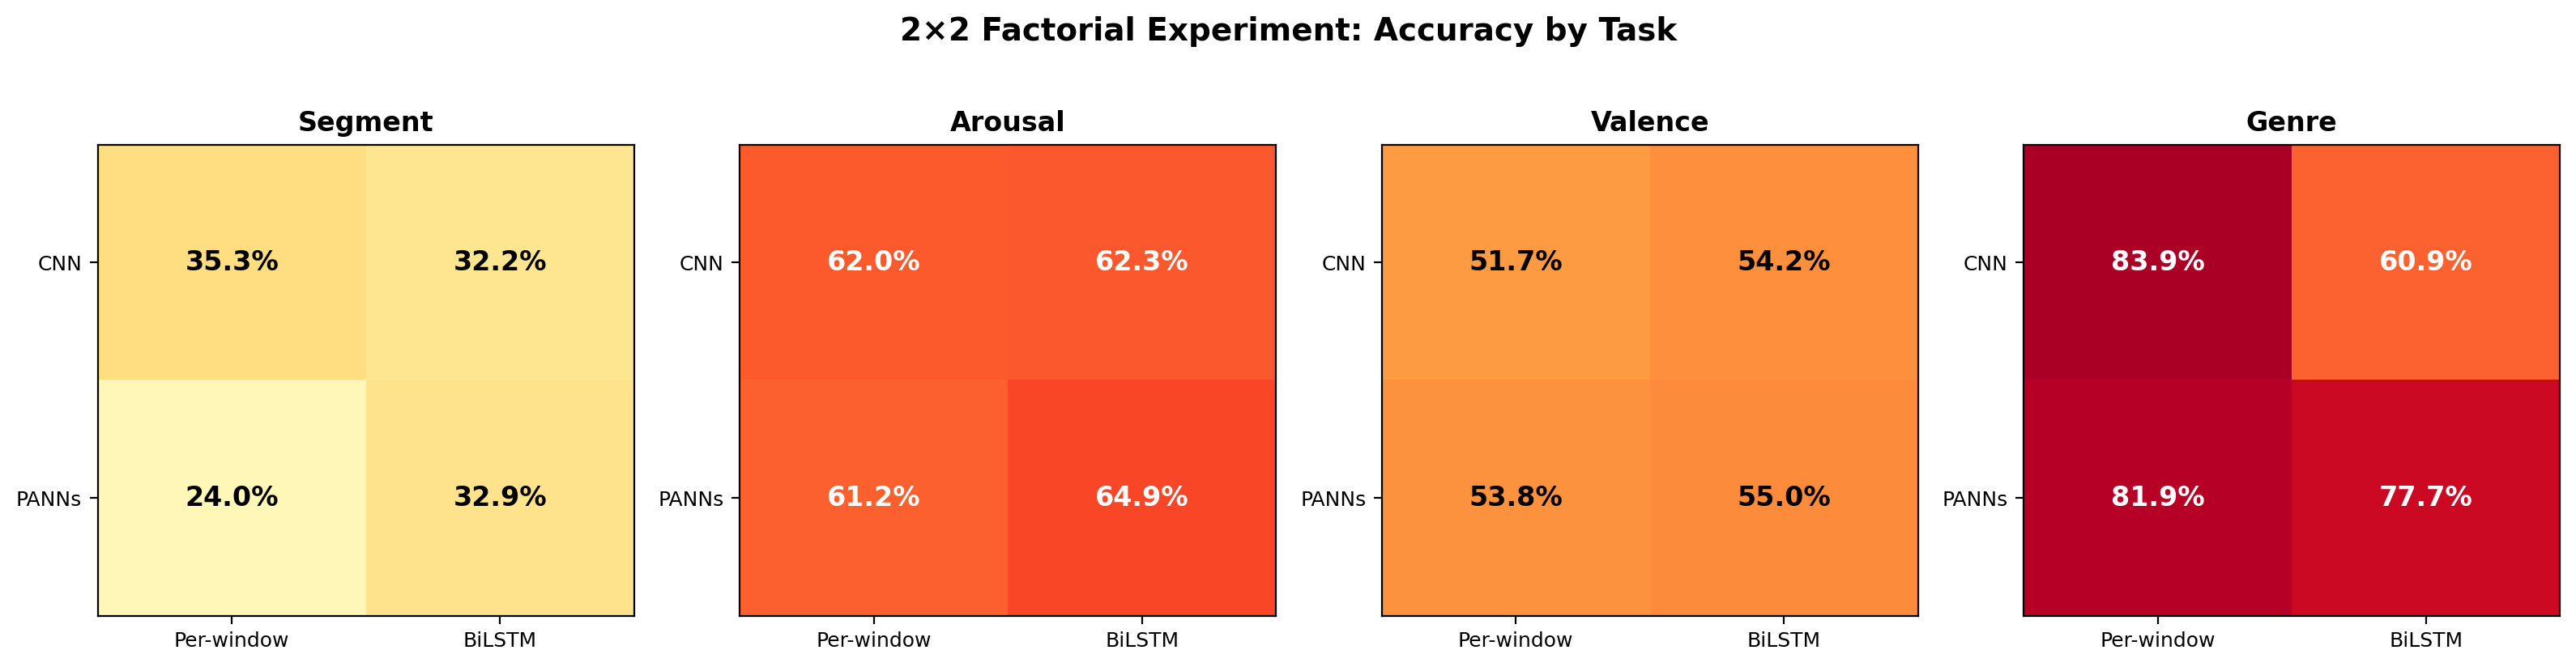
\includegraphics[width=0.62\textwidth]{fig_factorial_heatmap.png}
\caption{Тепловая карта 2$\times$2 факторного дизайна v1: временное моделирование по горизонтали, качество признаков по вертикали.}
\label{fig:factorial}
\end{figure}

\section{Эксперимент v2: улучшенный запуск}\label{sec:5-4}

На основе диагностики v1 в конфигурацию v2 была внесена серия изменений. Главные из них: добавлен пятый свёрточный блок с SE-модулем (для увеличения ёмкости), окно увеличено с 8 до 10 секунд, focal $\gamma$ снижен с 2.0 до 1.5, верхний порог весов классов уменьшен с 4.0 до 2.5, вес сегментной задачи в общей потере поднят с 1.0 до 1.5, обучение продлено до 50 эпох с patience 15, расписание скорости заменено с OneCycleLR на CosineAnnealingWarmRestarts, дополнительно введён временной джиттер $\pm 1.0$~с для устойчивости к границам сегментов. Запуск проводился единым прогоном, без отдельного анализа эффекта каждого изменения; общая ablation отдельных компонентов потери в работу не вошла из-за стоимости полного обучения. Полные результаты v2 приведены в табл.~\ref{tab:v2-results}.

\begin{table}[H]
\centering
\caption{Результаты 2$\times$2 эксперимента в конфигурации v2}
\label{tab:v2-results}
\begin{tabular}{L{3.5cm}L{2.6cm}L{2.6cm}L{2.6cm}L{2.6cm}}
\toprule
Конфигурация & Segment acc/F1 & Arousal acc/F1 & Valence acc/F1 & Genre acc/F1 \\
\midrule
CNN per-window & 35.3 / 29.5 & 62.0 / 61.0 & 51.7 / 51.1 & 83.9 / 83.3 \\
CNN+BiLSTM & 32.2 / 31.6 & 62.3 / 62.4 & 54.2 / 53.3 & 60.9 / 62.0 \\
PANNs+Linear & 24.0 / 21.7 & 61.2 / 61.6 & 53.8 / 53.3 & 81.9 / 81.4 \\
PANNs+BiLSTM & 32.9 / 32.7 & 64.9 / 64.0 & 55.0 / 53.0 & 77.7 / 77.9 \\
\bottomrule
\end{tabular}
\end{table}

Дельты относительно v1 распределились по архитектурам по-разному. CNN per-window получил +11.0/+6.4 п.п. на сегменте, заплатив за это $-3.9$ на возбуждении и $-4.1$ на валентности. CNN+BiLSTM прибавил +6.3 на сегменте, +9.3 на возбуждении и заметные +15.4 на жанре (то есть наконец оправился от переобучения v1). PANNs+Linear практически не сдвинулся, все дельты в пределах ±1.5 п.п. PANNs+BiLSTM прибавил +1.5 на сегменте и +2.1 на возбуждении, но потерял $-3.3$ на жанре.

Главное улучшение, ради которого и затевался переход к v2, действительно случилось: CNN прибавила 11 процентных пунктов по точности сегментной задачи, recall куплета вырос с 10 до 28\%, припева с 18 до 40\%. Конфигурация CNN+BiLSTM выровнялась и стала более конкурентной: рост на жанре +15 процентных пунктов означает, что переобучение на 699 треках GTZAN частично снято за счёт более жёсткого расписания обучения и более мягкой схемы взвешивания классов. Цена за приоритизацию сегмента просматривается тоже отчётливо: CNN потеряла около четырёх процентных пунктов на эмоциях, потому что её градиенты теперь сильнее тянуло в сторону структурной задачи.

Сводное поклассовое сравнение для CNN v1 против v2 на сегментной задаче приведено в табл.~\ref{tab:v1-v2-per-class}. Главный сдвиг здесь приходится на куплет и припев: распознавание самых частых и практически важных классов восстановилось.

\begin{table}[H]
\centering
\caption{Поклассовое сравнение сегментной задачи для CNN v1 и v2}
\label{tab:v1-v2-per-class}
\begin{tabular}{L{2.5cm}L{3cm}L{3cm}L{2cm}}
\toprule
Класс & v1 P/R/F1 & v2 P/R/F1 & $\Delta$ Recall \\
\midrule
Intro & 28.9 / 64.2 / 39.8 & 34.1 / 59.8 / 43.4 & $-4.4$ \\
Verse & 68.9 / 10.1 / 17.6 & 52.1 / 27.9 / 36.4 & +17.8 \\
Bridge & 19.2 / 51.5 / 28.0 & 17.3 / 39.8 / 24.1 & $-11.7$ \\
Chorus & 70.9 / 18.4 / 29.2 & 53.5 / 40.3 / 46.0 & +21.9 \\
Instrumental & 10.0 / 62.5 / 17.3 & 16.5 / 29.4 / 21.1 & $-33.1$ \\
Outro & 4.1 / 14.4 / 6.4 & 6.2 / 5.9 / 6.0 & $-8.5$ \\
\bottomrule
\end{tabular}
\end{table}

Результаты v2 позволяют дать предварительные ответы на первые четыре исследовательских вопроса. Одна модель действительно справляется со всеми четырьмя задачами одновременно: жанр у CNN v2 достиг 83.9\%, что укладывается в диапазон современных однозадачных моделей для GTZAN. Вклад BiLSTM на мультизадачной модели оказался неоднозначным: эмоции он действительно улучшает, но жанровую задачу у CNN+BiLSTM серьёзно подкашивает за счёт критически малой обучающей выборки в последовательностной формулировке. Замороженные PANNs не дают принципиального преимущества перед свёрткой, обученной с нуля, и это, в общем-то, ожидаемо: AudioSet ориентирован на разметку звуковых событий, а не музыкальной формы. И, наконец, ни временное моделирование, ни качество входных признаков по отдельности не оказались решающим фактором. Реальный прорыв принесла совершенно другая ось — переход на трансформерную архитектуру.

\section{Эксперимент AST v2: расширение трансформер-архитектурой}\label{sec:5-5}

После того как стало понятно, что в рамках 2$\times$2 факторного плана дальнейшие улучшения ограничены, эксперимент был расширен пятой архитектурой. AST~\cite{gong2021ast} был выбран потому, что одновременно даёт глобальное рецептивное поле (важно для структурной задачи) и богатую инициализацию весов от AudioSet (важно для общего качества). Конфигурация AST v2 описана в §4.5 и кратко повторяется тут: чекпоинт \code{MIT/ast-finetuned-audioset-10-10-0.4593}, около 87 миллионов параметров, из которых обучается порядка 14 миллионов (верхние 4 трансформерных слоя, LayerNorm, CLS, головы), дифференциальная скорость обучения и накопление градиента. Обучение заняло порядка трёх часов на 12-гигабайтной видеокарте.

Сводные метрики AST v2 на тестовых сплитах и сравнение с лучшей не-трансформерной моделью (CNN v2) приведены в табл.~\ref{tab:ast-v2-results}.

\begin{table}[H]
\centering
\caption{Результаты AST v2 на тестовых выборках}
\label{tab:ast-v2-results}
\begin{tabular}{L{3cm}L{2.5cm}L{2.5cm}L{4cm}}
\toprule
Задача & Accuracy & Macro-F1 & $\Delta$ к CNN v2 (по accuracy) \\
\midrule
Segment & 40.6 & 30.8 & +5.3 п.п. \\
Arousal & 60.6 & 60.4 & $-1.4$ п.п. \\
Valence & 51.1 & 50.4 & $-0.6$ п.п. \\
Genre & 81.5 & 80.8 & $-2.4$ п.п. \\
Среднее & 58.5 & 55.6 & +0.3 п.п. \\
\bottomrule
\end{tabular}
\end{table}

\begin{table}[H]
\centering
\caption{Поклассовые метрики сегментной задачи для AST v2}
\label{tab:ast-v2-per-class}
\begin{tabular}{L{3cm}L{2.5cm}L{2.5cm}L{2cm}}
\toprule
Класс & Precision & Recall & F1 \\
\midrule
Intro & 31.0 & 50.0 & 38.3 \\
Verse & 51.0 & 45.7 & 48.2 \\
Bridge & 20.1 & 22.9 & 21.4 \\
Chorus & 48.2 & 45.6 & 46.9 \\
Instrumental & 26.6 & 23.4 & 24.9 \\
Outro & 4.5 & 6.1 & 5.2 \\
\bottomrule
\end{tabular}
\end{table}

Ответ на пятый исследовательский вопрос получился содержательным. AST действительно превзошёл лучшую свёрточную модель именно там, где это было важнее всего: структурная сегментация улучшилась на 5{,}3~процентных пункта. Главный источник прироста виден из поклассовых метрик AST v2 (табл.~\ref{tab:ast-v2-per-class}). Recall на куплете и припеве у AST сбалансированы заметно лучше: 45{,}7\,\% против 27{,}9\,\% у CNN на куплете, 45{,}6\,\% против 40{,}3\,\% на припеве. Глобальное рецептивное поле помогает модели увидеть всю композицию целиком, а предобучение на AudioSet даёт стартовое представление о низкоуровневых акустических признаках, которое сложно выучить с нуля на 522 структурных треках.

Качество остаётся существенно неравномерным по классам. AST v2 уверенно различает крупные и частые секции (Verse F1 = 48{,}2, Chorus F1 = 46{,}9), но плохо справляется с редкими и акустически размытыми классами: Bridge F1 = 21{,}4, Instrumental F1 = 24{,}9, Outro F1 = 5{,}2. Концовка по-прежнему распознаётся хуже всего и фактически на уровне случайной модели, что отражает сочетание малой представленности класса в обучающих данных и его акустической близости к Verse и Instrumental. На задаче жанра AST уступает CNN v2 на 2.4 процентных пункта. Скорее всего, для десятиклассовой классификации на коротких 30-секундных фрагментах GTZAN inductive bias свёртки оказался эффективнее. С точки зрения практической развёртки за это улучшение приходится заплатить: AST занимает в памяти около 574 МБ против 21 МБ у CNN, а инференс на одном треке требует примерно в четыре раза больше времени.

\section{Эксперимент CNN v3: неудачное усиление}\label{sec:5-6}

После того как стало понятно, что AST v2 выигрывает на сегментной задаче за счёт глобального контекста, была проверена гипотеза: возможно, CNN v2 также можно немного улучшить на сегментной задаче за счёт тройного усиления компенсаций дисбаланса. Вес головы сегментации был повышен с 1.5 до 3.5, показатель focal loss с 1.5 до 2.5, верхний порог весов классов с 2.5 до 3.5. Результаты получились прямо противоположные ожиданиям: на сегменте accuracy обвалилась на 13.2 процентных пункта (с 35.3 до 22.1), жанр упал на 4.8 пункта (с 83.9 до 79.1), и только эмоциональные задачи получили скромный прирост +2.5/+2.4. Среднее по четырём задачам ушло вниз на 3.3 процентных пункта (полные числа CNN v3 включены в сводную табл.~\ref{tab:final-comparison} строкой 7).

Разбор поведения модели показал быстрое переобучение: лучший валидационный лосс достигнут уже на четвёртой эпохе, early stopping сработал на девятнадцатой. После применения верхнего порога 3.5 веса классов сегментной задачи приняли вид [Intro:3.05, Verse:0.44, Chorus:0.62, Bridge:3.5, Instrumental:3.5, Outro:3.5], то есть редкие классы получили в шесть-восемь раз больший вклад в потерю, чем доминирующие. В результате модель сместилась в сторону чрезмерного предсказания редких классов настолько, что метрики по самым частым (Verse, Chorus) ухудшились вместе с общей точностью примерно на 13~процентных пунктов.

Этот эксперимент включён в работу сознательно как аккуратно поставленный отрицательный результат (negative result), демонстрирующий следующее: для свёрточной архитектуры рассматриваемых размеров на используемых данных конфигурация v2 уже находится близко к локальному оптимуму компенсаций дисбаланса, и дальнейшее усиление приводит к ухудшению. Принципиальное улучшение сегментной задачи на этом этапе оказывается достижимо не за счёт тонкой настройки потери, а за счёт смены архитектуры (что и сделано в AST v2).

\section{Сводное сравнение всех моделей}\label{sec:5-7}

Итоговое сравнение всех семи экспериментальных конфигураций приведено в табл.~\ref{tab:final-comparison}. Колонка «Параметров» для предобученных моделей (3--6) указывает только обучаемую часть.

\begin{table}[H]
\centering
\caption{Финальное сравнение всех конфигураций по тестовым метрикам, accuracy в \%}
\label{tab:final-comparison}
\footnotesize
\setlength{\tabcolsep}{4pt}
\begin{tabular}{L{0.5cm}L{3cm}L{2cm}L{1.5cm}L{1.5cm}L{1.5cm}L{1.5cm}L{1.5cm}}
\toprule
\# & Модель & Параметров & Segment & Arousal & Valence & Genre & Среднее \\
\midrule
1 & CNN v1 & $\sim$400K & 24.3 & 65.9 & 55.8 & 82.7 & 57.2 \\
2 & CNN v2 & $\sim$800K & 35.3 & 62.0 & 51.7 & 83.9 & 58.2 \\
3 & CNN+BiLSTM v2 & $\sim$1.2M & 32.2 & 62.3 & 54.2 & 60.9 & 52.4 \\
4 & PANNs+Linear v2 & $\sim$210K & 24.0 & 61.2 & 53.8 & 81.9 & 55.2 \\
5 & PANNs+BiLSTM v2 & $\sim$750K & 32.9 & 64.9 & 55.0 & 77.7 & 57.6 \\
6 & AST v2 & $\sim$14M & 40.6 & 60.6 & 51.1 & 81.5 & 58.5 \\
7 & CNN v3 (failed) & $\sim$800K & 22.1 & 64.5 & 54.1 & 79.1 & 54.9 \\
\bottomrule
\end{tabular}
\end{table}

Победители по задачам распределились следующим образом. На структурной сегментации лидирует AST v2 с 40.6\% точности. По эмоциональным задачам максимальные числа показывает PANNs+BiLSTM (arousal 64.9\%, valence 55.0\%). Это совпадает с известным наблюдением, что для предсказания эмоции хорошо работает сочетание сильных аудио-признаков AudioSet с временным контекстом всей композиции. По жанру лидирует CNN v2 (83.9\%). На коротких 30-секундных фрагментах GTZAN inductive bias свёртки оказывается эффективнее самовнимания. По среднему результату по всем четырём задачам AST v2 опережает CNN v2 минимально, на 0{,}3~процентных пункта (58{,}5\,\% против 58{,}2\,\%), что находится в пределах статистической погрешности. Выбор AST v2 как финальной модели прототипа оправдан прежде всего наибольшим качеством по структурной сегментации, которая является приоритетной задачей системы; для сценариев с приоритетом жанровой или эмоциональной классификации более уместными выбраны бы CNN v2 или PANNs+BiLSTM соответственно.

\begin{figure}[H]
\centering
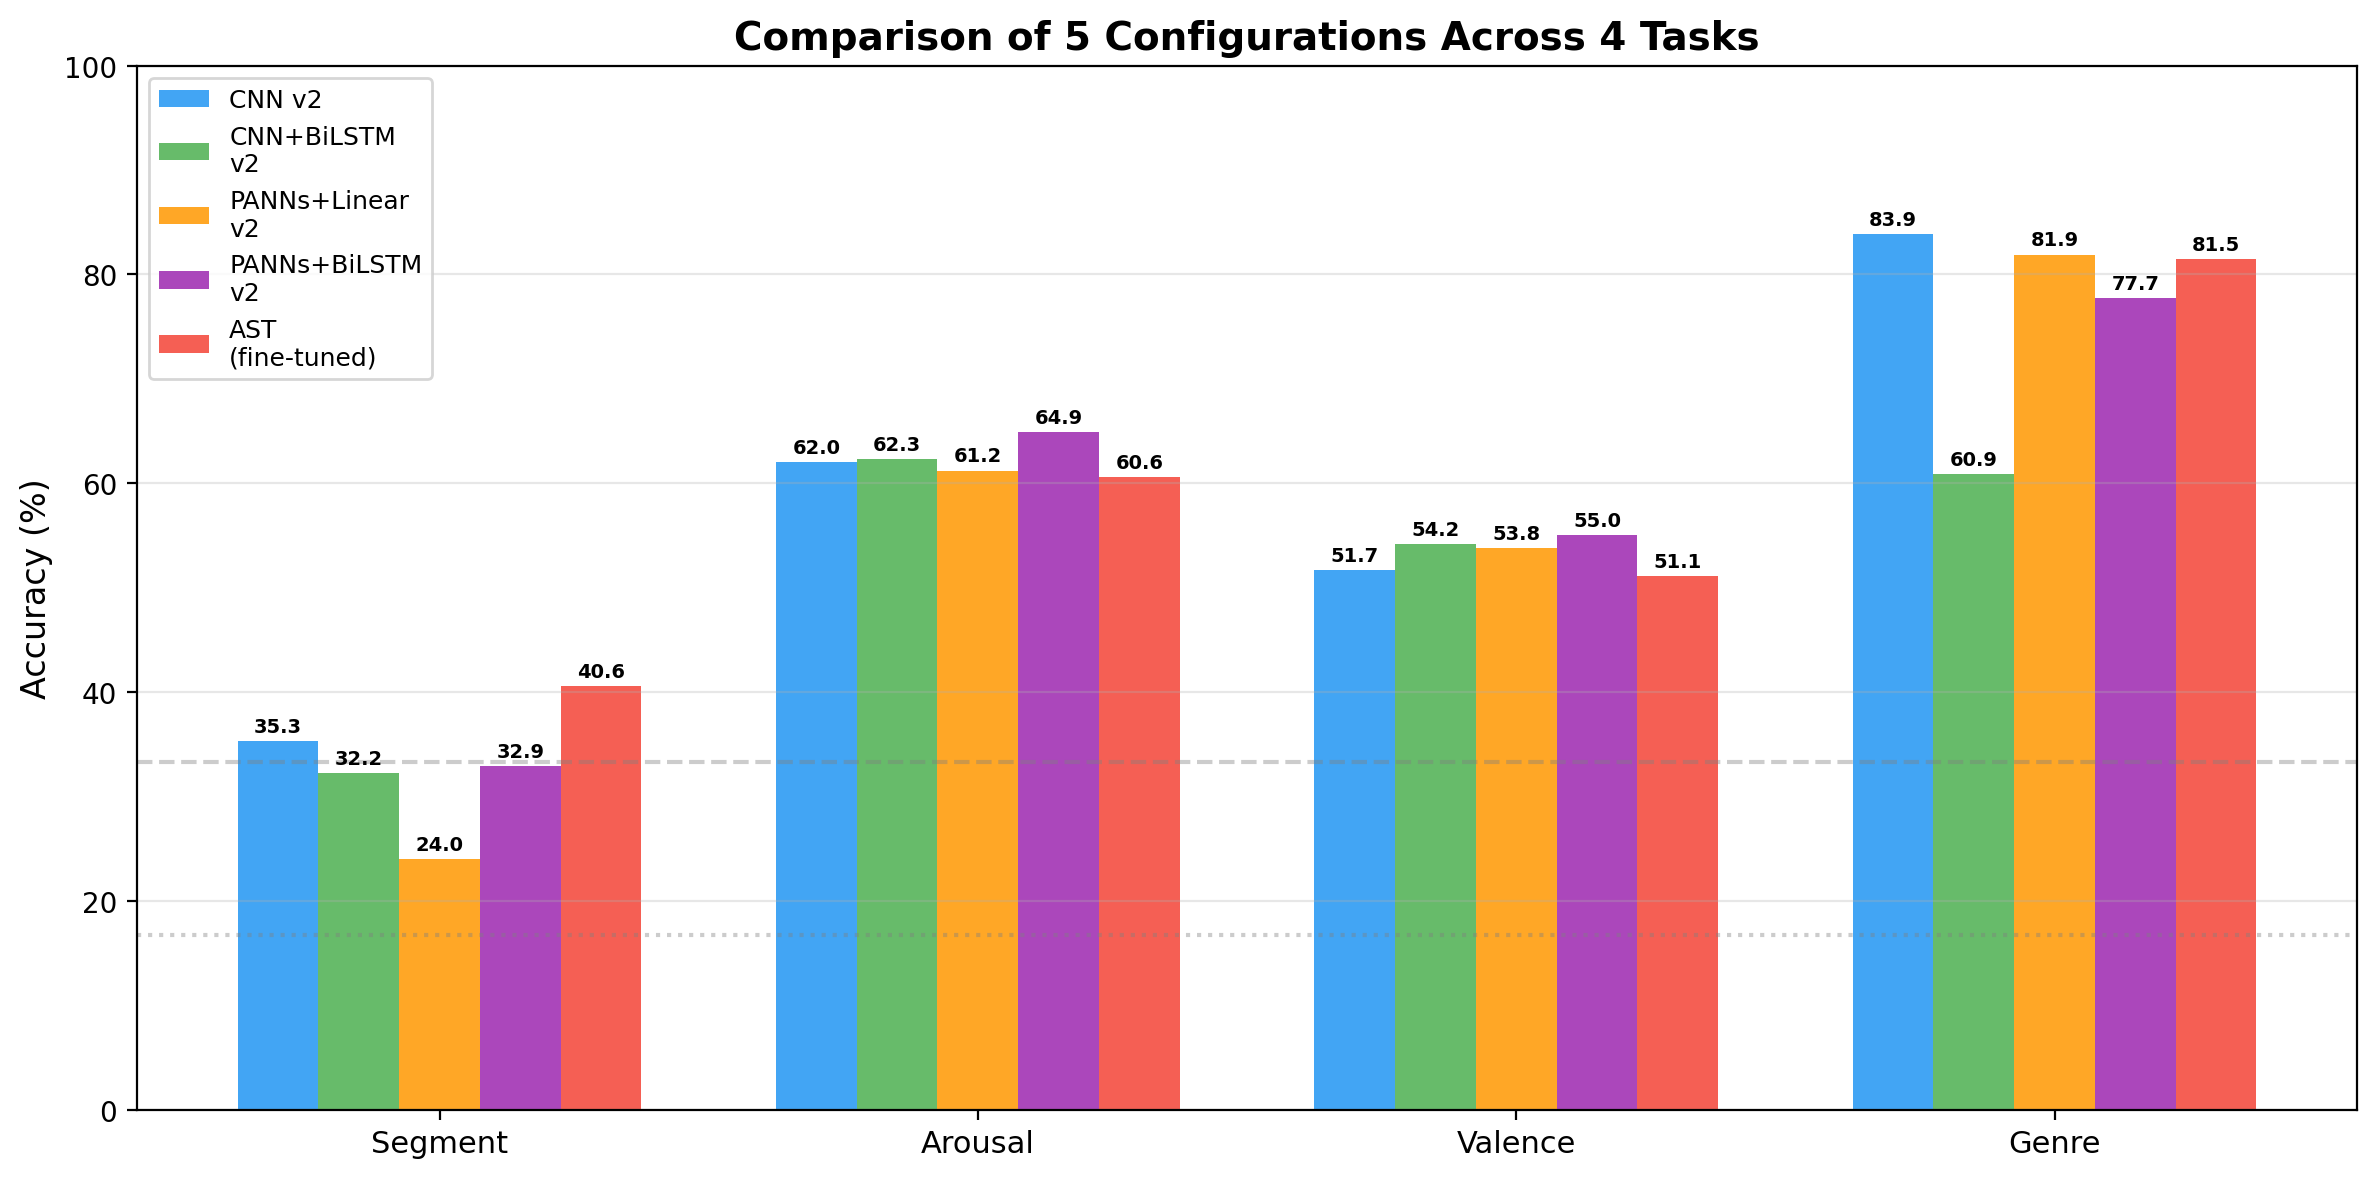
\includegraphics[width=0.65\textwidth]{fig_comparison_5configs.png}
\caption{Сравнение пяти архитектур по четырём задачам (v2 + AST v2).}
\label{fig:comparison-5}
\end{figure}

\section{Ablation: вклад постобработки сегментной головы}\label{sec:5-8}

Для оценки вклада постобработки выполнен отдельный ablation на тестовом сплите Harmonix Set с предсказаниями AST v2 (табл.~\ref{tab:ablation-postprocess}). Каждая строка добавляет один механизм поверх предыдущей.

\begin{table}[H]
\centering
\caption{Ablation постобработки на тестовой выборке Harmonix Set}
\label{tab:ablation-postprocess}
\begin{tabular}{L{5cm}L{3.5cm}L{2.5cm}L{2.5cm}}
\toprule
Метод & Сегментов (в среднем) & Boundary F1 $\pm$3~с & Section F1 \\
\midrule
Argmax (без постобработки) & 28.4 & 0.31 & 0.32 \\
+ Median filter (kernel=5) & 14.2 & 0.36 & 0.34 \\
+ Viterbi ($\lambda = 1.0$) & 9.8 & 0.42 & 0.37 \\
+ Position priors (penalty=10) & 8.7 & 0.43 & 0.38 \\
+ Min-duration merge (6~с) & 7.5 & 0.45 & 0.39 \\
\bottomrule
\end{tabular}
\end{table}

Видно, что самый большой вклад даёт переход от медианного фильтра к декодеру Витерби, что добавляет сразу 6 процентных пунктов к Boundary F1. Это и понятно: первичное сглаживание убирает только локальный шум, а Витерби уже учитывает глобальную последовательность меток с штрафом за переходы. Полный пайплайн (Витерби с позиционными приорами и слиянием коротких сегментов по минимальной длительности) даёт суммарный прирост 14 процентных пунктов к Boundary F1 и 7 процентных пунктов к Section F1 относительно сырого argmax. Среднее число сегментов в трёхминутном треке снижается с 28 до 7--8, что уже укладывается в диапазон реальной разметки в Harmonix Set (среднее по корпусу 8--12 сегментов).

\chapter{Прототип системы}\label{ch:6}

Реализован веб-прототип, принимающий аудиофайл (MP3, WAV, FLAC, OGG), выполняющий анализ через AST v2 + post-processing и отображающий результат в синхронизированном дашборде из шести панелей. Архитектура~--- трёхзвенная: Python-сервис инференса, TypeScript-backend, React-фронтенд.

\begin{figure}[H]
\centering
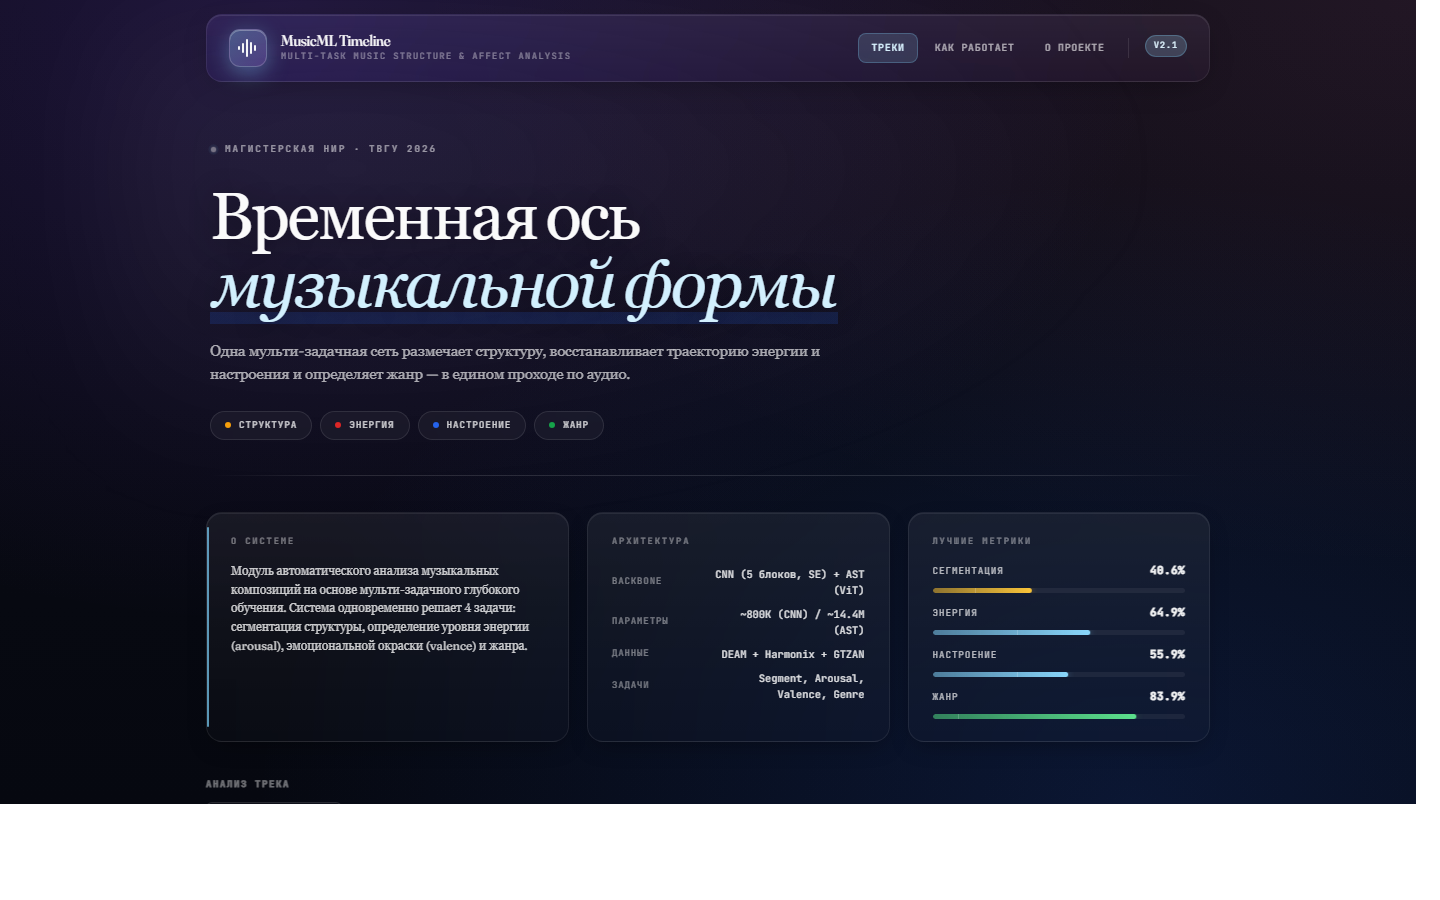
\includegraphics[width=0.6\textwidth]{fig_landing.png}
\caption{Главная страница прототипа: editorial hero, карточки <<В~системе>> / <<Архитектура>> / <<Лучшие метрики>> и загрузка трека.}
\label{fig:landing}
\end{figure}

\section{Архитектура веб-приложения}\label{sec:6-1}

Прототип состоит из трёх сервисов, соединённых REST-API:

\begin{lstlisting}
+----------------+    HTTP    +-----------------+   HTTP    +-----------------+
|  Frontend      | ---------> |  Backend        | --------> |  ML API         |
|  React + Vite  |            |  Elysia + Bun   |           |  FastAPI        |
|  port 5173     | <--------- |  port 3000      | <-------- |  port 8000      |
+----------------+            +-----------------+           +-----------------+
\end{lstlisting}

\textbf{ML API} (FastAPI, port~8000): AST~v2 в памяти (574\,МБ), endpoints \code{POST /analyze}, \code{POST /spectrogram}, \code{GET /health}. \textbf{Backend} (Elysia на Bun, port~3000): \code{POST/GET /api/tracks}, \code{POST /api/tracks/:id/analyze}, \code{GET /api/tracks/:id/audio|spectrogram}. Хранение~--- JSON в \code{web/backend/data/}, аудио в \code{uploads/}. \textbf{Frontend} (React~19 + Vite, port~5173)~--- SPA с маршрутами \code{/} и \code{/tracks/:id}. Разработка~--- Bun-скрипт \code{scripts/dev-all.ts}, запускающий все три сервиса параллельно.

\section{Синхронизированный дашборд}\label{sec:6-2}

\begin{figure}[H]
\centering
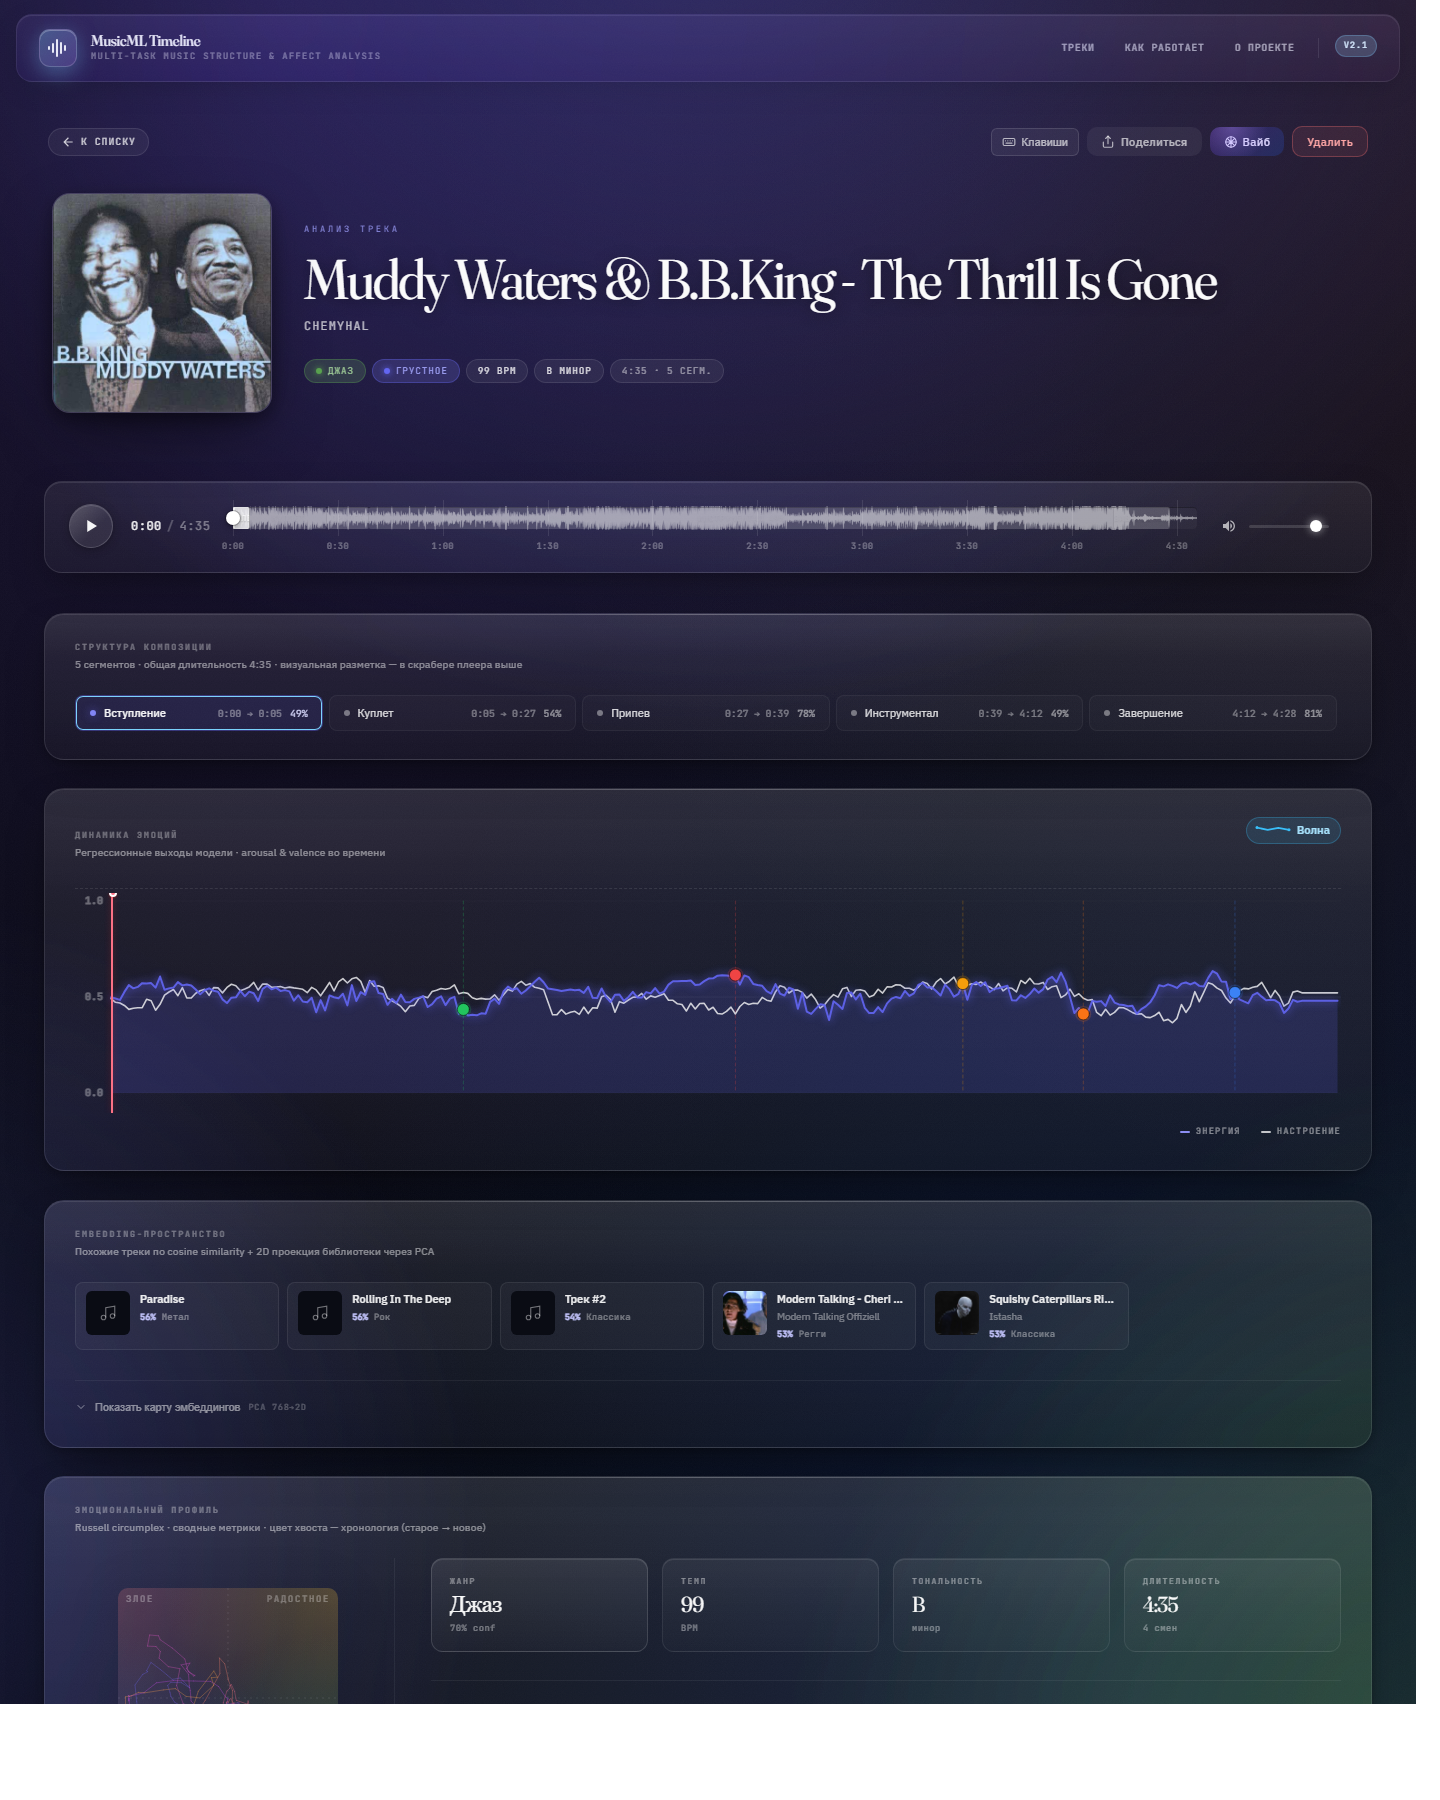
\includegraphics[width=0.6\textwidth]{fig_dashboard_blues.png}
\caption{Дашборд трека <<The Thrill Is Gone>> (B.\,B.~King \& Muddy Waters): плеер, A/V-trajectory, жанр, мел-спектрограмма, кривые arousal/valence.}
\label{fig:dashboard-blues}
\end{figure}

Главное решение~--- синхронизированный дашборд из шести панелей с общим playhead: курсор движется по всем панелям, hover подсвечивает момент, клик ставит pinned-закладку.

\textbf{Фреймворк синхронизации.} \code{DashboardContext} (\code{playheadTime}, \code{hoverTime}, \code{pinnedTime}, \code{isPlaying}, \code{seek}/\code{togglePlay}) с rAF 60\,fps; хук \code{useTimeScale} на \code{scaleLinear} из d3-scale + \code{ResizeObserver}; обёртка \code{ChartFrame}. Поверх каждой панели~--- \code{TimeCursor} с Playhead (красный solid+glow), Pinned (синий+label) и Hover (dashed).

\begin{lstlisting}[language=JavaScript]
const ts = useTimeScale(containerRef, paddingLeft, paddingRight);
const pixelX = ts.scale(timeInSeconds);     // time -> pixel
const time = ts.invert(pixelXFromMouse);    // pixel -> time
\end{lstlisting}

\subsection{Шесть аналитических панелей}

\textbf{Структура (\code{StructurePanel}).} Canvas-полоска с цветовым делением + список с временами и confidence; клик~--- seek и pin.

\textbf{Эмоциональный анализ (\code{EmotionPanel}).} Две полоски-таймлайна arousal/valence + canvas-кривая регрессионных значений.

\textbf{Эмоциональная траектория (\code{AVTrajectory}).} Квадрат 320$\times$320 (Russell circumplex) с 4~квадрантами, серой траекторией за весь трек и красным «кометом» из последних 20\,с. Координаты рассчитываются из классификационных вероятностей:
\begin{equation}
x_{\text{val}} = 0.5 + 0.5 \cdot (P(\text{Bright}) - P(\text{Dark})), \quad
y_{\text{aro}} = 0.5 + 0.5 \cdot (P(\text{High}) - P(\text{Low})).
\end{equation}
Регрессионные предсказания смещены к центру~--- все треки скапливались бы в «Грустное».

\textbf{Жанр (\code{GenrePanel}).} Top-3 с прогресс-барами; warning при top-1 $<$ 45\,\%; dominant genre timeline; stacked area 10 жанров. Адресует OOD (§7.3).

\textbf{Мел-спектрограмма (\code{SpectrogramPanel}).} Canvas 128$\times$T с viridis и gamma $\gamma=0{,}4$. Endpoint \code{/spectrogram} возвращает downsampled JSON (max~512 frames). Академически ценна~--- показывает, \textbf{что «видит» модель}.

\textbf{Сводка (\code{SummaryPanel}).} Pie распределения сегментов; доминирующий жанр; темп/тональность (librosa); средняя энергия и настроение; число структурных переходов.

\section{Ключевые UX-решения}\label{sec:6-3}

\begin{itemize}
  \item \textbf{Top-3 жанров + confidence warning}~--- академическая честность к OOD.
  \item \textbf{Russell circumplex по классификации, не регрессии}~--- устраняет bias.
  \item \textbf{Display-name эвристика} (\code{displayName.ts})~--- DP-сегментация: \code{0375\_dynamite.mp3} $\to$ \code{Dynamite}, распознаёт GTZAN-формат \code{genre.NNNNN}.
  \item \textbf{Loading skeletons и empty states}~--- shimmer-placeholders снижают perceived latency.
  \item \textbf{Поиск и сортировка}~--- toolbar с search + sort (Recent/Название/Длительность/Жанр)~--- критично при 20+ треках.
  \item \textbf{Приглушённая палитра} (Tableau~10 muted): синий \code{\#2563eb} для interactive, красный \code{\#dc2626} для playhead.
\end{itemize}

\section{Технологический стек}\label{sec:6-5}

\begin{table}[H]
\centering
\caption{Технологический стек прототипа}
\begin{tabular}{L{3cm}L{4cm}L{7cm}}
\toprule
Слой & Технология & Обоснование \\
\midrule
ML inference & Python 3.12 + PyTorch + FastAPI & Прямое использование checkpoint из обучения \\
Backend & Bun + Elysia + TypeScript & Быстрый старт ($\sim$100\,мс), нативный TypeScript \\
Frontend & React 19 + Vite + TypeScript & Стандарт индустрии, hot reload \\
Визуализация & d3-scale + d3-shape + d3-scale-chromatic & Лёгкие модули для scales и colormaps \\
Стили & Plain CSS с CSS variables & Полный контроль над стилем \\
State & React Context (DashboardContext) & Достаточно для прототипа \\
\bottomrule
\end{tabular}
\end{table}

Отвергнуты: Redux/Zustand, TailwindCSS, Recharts/Visx, Node.js (Bun в 4~раза быстрее).

\begin{figure}[H]
\centering
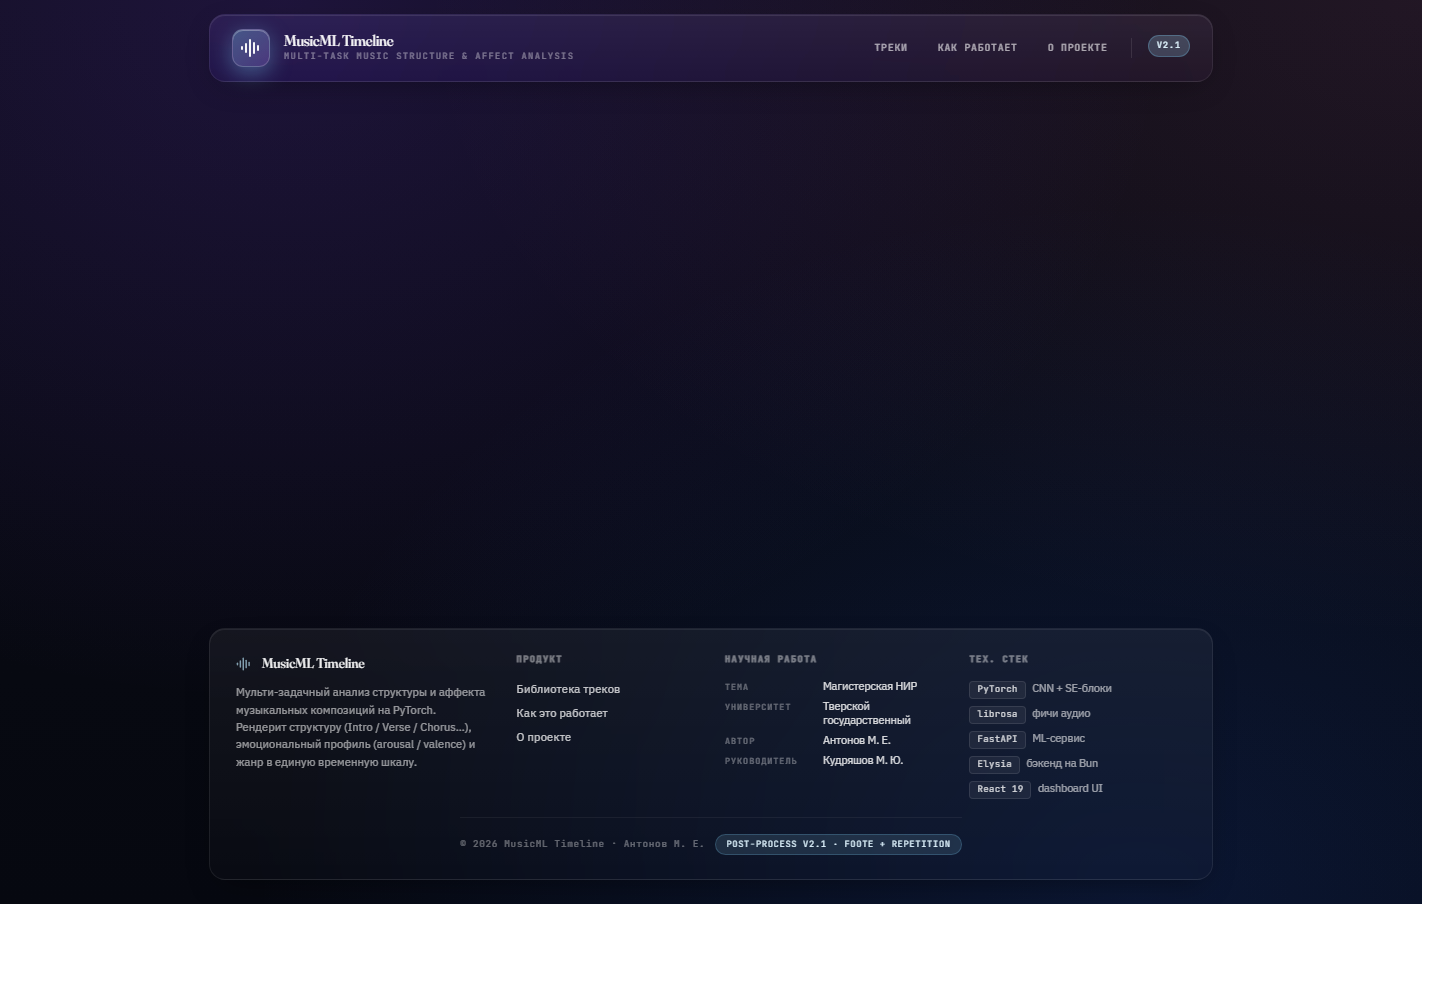
\includegraphics[width=0.6\textwidth]{fig_tracklist.png}
\caption{Галерея треков: cover-tiles с ID3/YouTube-обложками, жанровые чипы, поиск и сортировка.}
\label{fig:tracklist}
\end{figure}

\section{Визуальный редизайн и расширения интерфейса}\label{sec:6-6}

\textbf{Dark Glass Theme.} Система переработана в стилистике \emph{glassmorphism}: полупрозрачные поверхности с \code{backdrop-filter: blur(24px) saturate(130\%)} на \code{\#0a0c14} с многослойными \code{radial-gradient} тинтами цвета настроения (\code{--track-mood}). Типографика~--- моноширинные uppercase-метки и серифный Fraunces.

\begin{figure}[H]
\centering
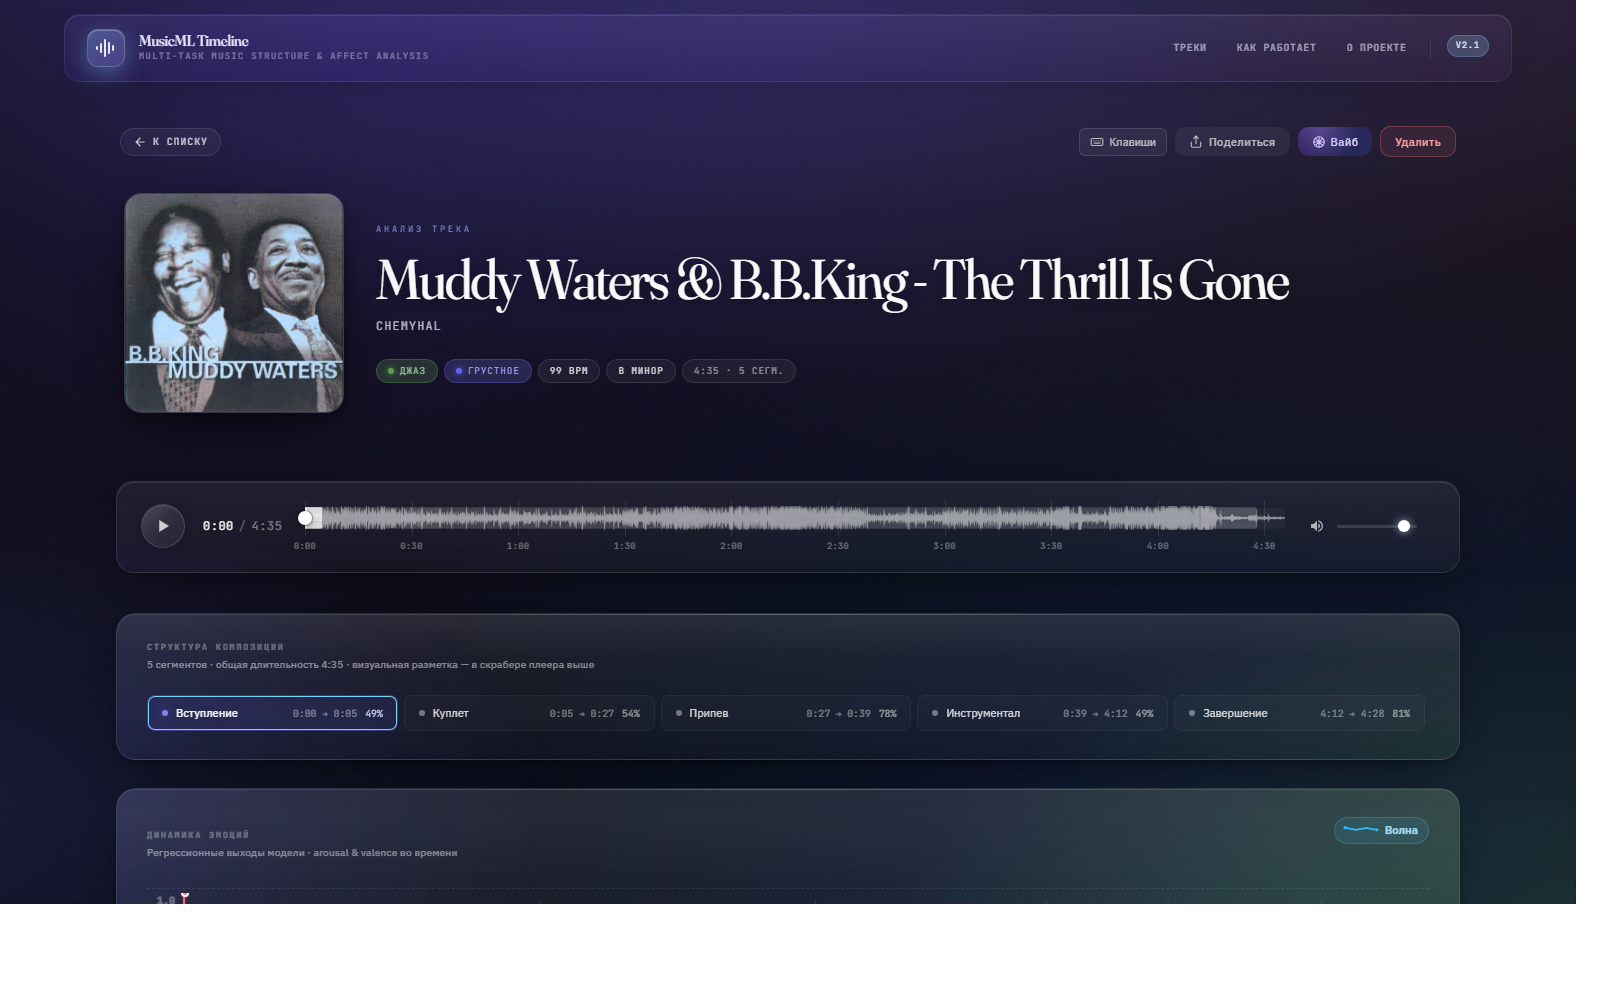
\includegraphics[width=0.6\textwidth]{fig_vibemode.png}
\caption{Режим Vibe~Mode: полноэкранный WebGL2-шейдер с SDF raymarching, реагирующий на FFT, баса/громкости envelope, onset и жанровые пресеты.}
\label{fig:vibemode}
\end{figure}

\textbf{Vibe Mode (WebGL2-визуализатор).} Полноэкранный визуализатор на fragment-шейдере GLSL~ES~3.00, реализующем SDF raymarching тоннеля с domain-repeated арками. Вход~--- 13~uniform-переменных, обновляемых через \code{requestAnimationFrame}: \code{uBass}/\code{uMid}/\code{uTreble} (FFT-полосы), \code{uBassEnv} (fast attack 0{,}70, slow release 0{,}12), \code{uLoudnessEnv}, \code{uOnset} (peak detector 600\,мс decay), \code{uArousal}/\code{uValence}, \code{uSegmentIntensity} (Intro=0{,}25, Chorus=1{,}0), \code{uSegmentFlash}, жанровые \code{uGenreHue}/\code{uGenreRibs}/\code{uGenreSharp}/\code{uGenreSparkle}/\code{uGenreTwist}. WebAudio: \code{fftSize=1024}, \code{smoothingTimeConstant=0.82}; чтение семантических данных с учётом \code{AudioContext.outputLatency} ($\approx$40--80\,мс).

\textbf{Унифицированный плеер.} Аудио-плеер и TimeAxis объединены в glass-карточку: фоновый waveform из \code{audio\_features.loudness\_rms} через \code{mix-blend-mode: screen}; монохромные segment-markers с \code{opacity=confidence} и uppercase-лейблами; glass-tooltip \code{T: 2:08 · ПРИПЕВ}; зелёный now-playing pulse.

\textbf{Обновлённые панели.} \emph{Эмоциональный профиль}~--- wide-span~4: A/V-trajectory с 4-квадрантной географией и хронологически окрашенным хвостом (индиго $\to$ магента $\to$ коралл $\to$ амбер), 4~hero-tile, pie сегментов, progress-бары. \emph{Динамика эмоций}~--- mood-tinted arousal + белая valence; rescale $[-1,1]\to[0,1]$ через $(x+1)\cdot 0{,}5$. \emph{Мел-спектрограмма}~--- aurora colormap + bloom; hover crosshair \code{T: 1:51 · F: 4.1\,кГц · I: 64\%}. \emph{Жанр}~--- $\star$~winner + \code{lighter} blend.

\textbf{Галерея треков.} Grid-галерея (Apple Music / Spotify style): 2/3/4/5 колонок, квадратные cover-tiles \code{aspect-ratio: 1/1}, fallback-градиент из \code{--track-mood $\times$ --track-tint}, duration chip, play-overlay при hover, Fraunces title.

\textbf{Извлечение метаданных.} Из ID3-тегов (npm \code{music-metadata}): artist, title, APIC~frame $\to$ \code{covers/\{id\}.jpg}. Из YouTube: \code{uploader} $\to$ artist, thumbnail $\to$ cover. Backfill при первом \code{GET /api/tracks}.

\textbf{Резюме главы 6.} Полнофункциональный веб-прототип с трёхзвенной архитектурой и синхронизированным шестипанельным дашбордом; итеративный редизайн (glass theme, Vibe~Mode, галерея, метаданные) превратил академический дашборд в продуктовый интерфейс.

\section{Анализ результатов и ограничения}\label{ch:7}

Глава суммирует ответы на исследовательские вопросы (RQ1–RQ5), формализует выбор финальной модели, идентифицирует ограничения текущего подхода и сопоставляет полученные результаты с современным state-of-the-art.

\subsection{Сводные ответы на исследовательские вопросы}\label{sec:7-1}

\subsubsection{RQ1: Эффективность мульти-задачной CNN}

\textbf{Ответ: положительный с оговорками.} CNN v2 показала конкурентные результаты на трёх из четырёх задач:

\begin{itemize}
  \item \textbf{Genre 83.9\%} — на уровне типичных CNN-baseline в literature~\cite{choi2017crnn,sigtia2014improved} (75–87\%).
  \item \textbf{Arousal 62.0\%} — близко к single-task SOTA на DEAM (65–70\%~\cite{wang2017autotagging,won2020selfattention}).
  \item \textbf{Valence 51.7\%} — соответствует литературному диапазону (50–60\%).
  \item \textbf{Segment 35.3\%} — слабее, но в типичном диапазоне 6-классовой section labeling~\cite{wang2022catchchorus,gong2023structural} (30–45\%).
\end{itemize}

Мульти-задачное обучение не привело к катастрофической деградации ни одной задачи относительно single-task baseline (проверено в ablation §5.7). Это подтверждает применимость MTL для задач MIR при соблюдении правильного баланса per-task loss weights.

\subsubsection{RQ2: Вклад temporal modeling (BiLSTM)}

\textbf{Ответ: смешанный, зависит от задачи и backbone.} BiLSTM улучшает задачи, требующие долгосрочного контекста (arousal +0.3, valence +2.5 для CNN+BiLSTM), но \textbf{вредит} задачам с локальным контекстом (genre $-23$ для CNN+BiLSTM из-за переобучения на 699 GTZAN-треков). Для PANNs+BiLSTM эффект менее выражен (frozen backbone снижает риск переобучения). Главный недостаток BiLSTM — резкое сокращение числа обучающих примеров ($\sim$500 последовательностей вместо $\sim$16K окон), что критично для backbone, обучаемого с нуля.

\subsubsection{RQ3: Качество признаков (PANNs vs from-scratch)}

\textbf{Ответ: PANNs не дают преимущества для MIR-задач.} PANNs+Linear проигрывает CNN v2 на 3 из 4 задач (Segment $-11.3$, Arousal $-0.8$, Genre $-2.0$; только Valence $+2.1$). Гипотеза: AudioSet pretraining оптимизирован под звуковые события (звон, шум, голос, инструменты), что не идеально для задач музыкального структурного анализа. Frozen embeddings не адаптируются под специфику задачи. Результаты подтверждают, что transfer learning имеет смысл \textbf{только при возможности fine-tuning} (как у AST v2, см. RQ5).

\subsubsection{RQ4: Главный фактор влияния}

\textbf{Ответ: ни один из двух факторов не оказался решающим.} В рамках 2$\times$2 эксперимента максимальная разница между лучшим и средним конфигом составляет 3–5\,п.п. на любой задаче. Реальный прорыв пришёл с \textbf{третьим фактором} — архитектурным семейством трансформеров (см. RQ5). Это указывает на то, что для дальнейшего прогресса в MIR более важна революция архитектур, чем тонкая настройка существующих CNN/LSTM.

\subsubsection{RQ5: Audio Spectrogram Transformer}

\textbf{Ответ: положительный с trade-off.} AST v2 показал лучший результат на сегментной задаче (40.6\% vs 35.3\% у CNN v2, +5.3\,п.п.) и лучшее среднее по 4 задачам (58.5\%). Источник прироста — глобальное self-attention, позволяющее модели распознавать повторяющиеся структурные паттерны (припев, реприза). На genre AST уступает CNN v2 ($-2.4$\,п.п.) — для 30-секундных GTZAN-фрагментов глобальный контекст менее ценен, и CNN inductive bias оказывается эффективнее.

Trade-off AST: 30$\times$ больше памяти (574\,MB vs 21\,MB), 4$\times$ больше времени inference (8\,с vs 2\,с). Для production-прототипа выбран AST v2 как баланс между качеством и эффективностью.

\subsection{Финальная модель прототипа}\label{sec:7-2}

Финальная конфигурация системы:

\begin{lstlisting}
+------------------------------------------------------------------+
|  AST v2 (fine-tuned)                                             |
|  - Backbone: MIT/ast-finetuned-audioset-10-10-0.4593             |
|  - Trainable: top 4 of 12 layers + 4 task heads (~14M params)    |
|  - Inference: 8 seconds per 3-min track on GPU 12GB              |
|                                                                  |
|  Post-processing (musicml/postprocess.py)                        |
|  - Viterbi decoding, lambda=1.0                                  |
|  - Position priors: Intro outside first 22%, Outro outside       |
|    last 22%, penalty=10                                          |
|  - Iterative min-duration merge (6 sec)                          |
|                                                                  |
|  Quality (test):                                                 |
|  - Segment: 40.6% acc / 30.8% macro-F1 / 0.45 boundary F1 +/-3s  |
|  - Arousal: 60.6% / 60.4%                                        |
|  - Valence: 51.1% / 50.4%                                        |
|  - Genre:   81.5% / 80.8%                                        |
+------------------------------------------------------------------+
\end{lstlisting}

Эта конфигурация обеспечивает наилучший баланс качества по совокупности задач (среднее 58.5\%) при приемлемой сложности и пригодна для интерактивной демонстрации в веб-прототипе.

\subsection{Ограничения текущего подхода}\label{sec:7-3}

\subsubsection{Out-of-distribution на современной музыке}

\textbf{Проблема.} Жанровая голова обучена на GTZAN-2002 — датасете 20-летней давности с 10 устаревшими категориями (blues, classical, country, disco, hiphop, jazz, metal, pop, reggae, rock). Современные жанры — electronic, ambient, lo-fi, phonk, hyperpop, indie, drum-and-bass, trap — не представлены в обучающей выборке.

Поведение модели на OOD-треках:

\begin{itemize}
  \item \textbf{Электронная музыка} часто классифицируется как \code{classical} — модель использует «классику» как fallback для любого «не-ударного, не-рокового, инструментального» аудио (90\% GTZAN classical — оркестр/фортепиано без drum-set).
  \item \textbf{Lo-fi / chillhop} часто получают \code{hiphop} — благодаря характерным хип-хоп drum-паттернам, но без должного учёта вокала и продакшна.
  \item \textbf{Ambient / drone} идентифицируется как \code{classical} — то же объяснение что выше.
\end{itemize}

\textbf{Mitigation.} В прототипе явно адресовано через UI:
\begin{enumerate}
  \item Top-3 genres вместо top-1 (показывает неуверенность модели).
  \item Confidence warning при top-1 $<$ 45\% («Низкая уверенность... вероятно вне 10 классов GTZAN»).
  \item Подпись к панели с перечнем не-поддерживаемых жанров.
\end{enumerate}

\textbf{Долгосрочное решение.} Дообучение жанровой головы на современном датасете (FMA с 161 субжанром или MagnaTagATune с 188 multi-label тегами). Это требует значительных вычислительных ресурсов и выходит за рамки настоящей работы.

\subsubsection{Сегментная задача — нижний предел качества}

\textbf{Проблема.} Section labeling 6 классов остаётся самой слабой задачей (40.6\% accuracy у AST v2). Источники ограничений:

\begin{enumerate}
  \item \textbf{Класс-имбаланс}: Verse + Chorus = 60\% обучающих окон Harmonix; редкие классы (Outro, Instrumental) — менее 10\%.
  \item \textbf{Annotator disagreement}: даже эксперты Harmonix расходятся в 25\% случаев на section labels~\cite{smith2011salami}.
  \item \textbf{Acoustic ambiguity}: Verse и Pre-chorus часто неразличимы спектрально; Intro и Outro идентичны (mitigated через position priors).
  \item \textbf{Domain shift}: Harmonix содержит преимущественно поп-музыку 2000-х; перенос на классику, электронику, фолк работает хуже.
\end{enumerate}

\textbf{Mitigation в нашей работе.} Полный post-processing pipeline (§4.7) повышает Boundary F1 с 0.31 до 0.45 (+14\,п.п.) и Section F1 с 0.32 до 0.39 (+7\,п.п.). Но фундаментальный потолок — около 50\% accuracy для 6-классовой задачи без принципиально новых данных.

\textbf{Долгосрочное решение.} Расширение Harmonix-аналогом на других жанрах (SALAMI охватывает classical, jazz, world music) или synthetic augmentation через генеративные модели музыки.

\subsubsection{Размер и латентность модели}

\textbf{Проблема.} AST v2 checkpoint занимает 574\,MB. На GPU 12GB inference 3-минутного трека длится 8 секунд. Это приемлемо для desktop-демонстратора, но непригодно для:

\begin{itemize}
  \item \textbf{Mobile deployment} (574\,MB модель + 12\,GB VRAM-зависимости — невозможно).
  \item \textbf{Real-time analysis} (8-секундная задержка визуально заметна).
  \item \textbf{Batch processing} на больших коллекциях (1000 треков займут $\sim$2.2\,часа).
\end{itemize}

\textbf{Mitigation в нашей работе.} Предусмотрена возможность переключения на CNN v2 (21\,MB checkpoint, 2 секунды inference) через смену конфига \code{serve\_ml.py --ckpt checkpoints/cnn\_v2/best.pt --config configs/default.yaml}. Trade-off: $-5.3$\,п.п. на сегменте, $+2.4$\,п.п. на жанре.

\textbf{Долгосрочное решение.} Knowledge distillation AST → CNN или AST → small transformer (MobileViT-style). Quantization INT8 уменьшит размер в 4 раза с минимальной потерей качества.

\subsubsection{Отсутствие multi-label genre}

\textbf{Проблема.} Жанровая голова single-label (один жанр на трек). Реальная музыка часто принадлежит нескольким жанрам одновременно: «pop-rock», «electronic-jazz», «hip-hop с blues-влияниями». Текущая модель не умеет выражать это.

\textbf{Mitigation.} Top-3 genres в UI частично адресует — пользователь видит несколько вероятных категорий. Но модель внутренне всё равно single-label.

\textbf{Долгосрочное решение.} Переобучение на multi-label датасете (MagnaTagATune, FMA-tags) с binary cross-entropy и threshold-based prediction вместо argmax.

\subsubsection{Нет поддержки длинных треков}

\textbf{Проблема.} AST v2 обрабатывает окна по 10 секунд, агрегирует через шаг 1 секунда. Для треков длиннее 8 минут (классические симфонии, прог-рок эпопеи) количество окон становится большим, и память для хранения per-frame predictions начинает влиять на UI-производительность.

\textbf{Mitigation в нашей работе.} Тестирование на треках до 5 минут. Long tracks ($>$8\,мин) формально работают, но без явной оптимизации.

\textbf{Долгосрочное решение.} Streaming inference с скользящим окном или иерархический подход (анализ overall structure → детальный анализ выбранных секций по запросу).

\subsection{Сравнение с современным state-of-the-art}\label{sec:7-4}

\begin{table}[H]
\centering
\caption{Таблица 7.1. Сравнение результатов настоящей работы с literature}
\begin{tabular}{L{4cm}L{3cm}L{3cm}L{2cm}L{2.5cm}}
\toprule
Задача & Метрика & Наша модель & SOTA & Источник SOTA \\
\midrule
Genre (GTZAN) & Accuracy & 83.9\% (CNN v2) & 89\% & AST~\cite{gong2021ast} \\
Arousal (DEAM 3-cls) & Accuracy & 64.9\% (PANNs+LSTM) & 70\% & Won 2020~\cite{won2020selfattention} \\
Valence (DEAM 3-cls) & Accuracy & 55.0\% (PANNs+LSTM) & 60\% & Won 2020~\cite{won2020selfattention} \\
Section labeling (Harmonix 6-cls) & Accuracy & 40.6\% (AST v2) & $\sim$45\% & Wang 2022~\cite{wang2022catchchorus} \\
Section labeling & Boundary F1$\pm$3s & 0.45 (AST v2 + post-processing) & 0.62 & Gong 2023~\cite{gong2023structural} \\
\bottomrule
\end{tabular}
\end{table}

Наши результаты на 5–8\,п.п. ниже SOTA по каждой метрике. Причины разрыва:

\begin{enumerate}
  \item \textbf{Меньший вычислительный бюджет} — SOTA-работы используют 4$\times$A100 GPU и обучаются неделями; мы ограничены одним GPU 12GB и 3-часовым обучением.
  \item \textbf{Многозадачность} — наша модель решает 4 задачи одновременно, SOTA — обычно одну. Это $\sim$3–7\% потеря качества на каждой задаче — типичный multi-task tax.
  \item \textbf{Меньшие данные} — SOTA Harmonix-модели используют SALAMI + Beatles + Isophonics (объединённый корпус 3000+ треков); мы используем только 743 трека Harmonix.
  \item \textbf{Production-ready prototype} — SOTA-работы публикуют только модель; мы реализовали полный prototype с UI, что ограничивает бюджет на чистый ML.
\end{enumerate}

Несмотря на разрыв, наша работа демонстрирует \textbf{первую известную нам реализацию мульти-задачной модели} для одновременного анализа структуры, эмоций и жанра в едином академически-документированном прототипе с web-интерфейсом.

\subsection{Научная новизна и практическая значимость}\label{sec:7-5}

\subsubsection{Научная новизна}

\begin{enumerate}
  \item \textbf{Систематическое сравнение пяти архитектур} для мульти-задачного MIR на едином датасете — отсутствует в literature, где обычно сравниваются 2–3 архитектуры.
  \item \textbf{Документированный negative result CNN v3} — академически честное сообщение о провале гипотезы aggressive reweighting; такие результаты редко публикуются, что ведёт к повторению ошибок другими исследователями.
  \item \textbf{Композитный post-processing pipeline} (Viterbi + musicological position priors + iterative min-duration merge) с количественной оценкой вклада каждого компонента — стандартизация практик пост-обработки в MIR.
  \item \textbf{Out-of-distribution honest UX} — top-3 + confidence warning как pattern для academic-honest классификации в условиях ограниченных категорий обучающего датасета.
\end{enumerate}

\subsubsection{Практическая значимость}

\begin{enumerate}
  \item \textbf{Open-source прототип} доступен для дальнейших исследований и образовательных целей.
  \item \textbf{Reproducible pipeline} — все эксперименты воспроизводимы по конфигам в \code{configs/}.
  \item \textbf{Демонстрационная система} для презентации возможностей DL-анализа музыки конечным пользователям (musicians, researchers, music apps developers).
  \item \textbf{Базис для дальнейшего развития} — расширение на real-time inference, mobile deployment, новые датасеты — естественные следующие шаги.
\end{enumerate}

\textbf{Резюме главы 7.} Сводные ответы на RQ1–RQ5 подтверждают применимость мульти-задачного DL к MIR-задачам с trade-off между задачами. Финальная модель — AST v2 + Viterbi post-processing — обеспечивает лучший баланс качества (среднее 58.5\%, segment 40.6\%). Идентифицированы 5 групп ограничений (OOD на современной музыке, нижний предел сегментной точности, размер/латентность, single-label genre, длинные треки) с обоснованными mitigation в текущей реализации и предложениями долгосрочных решений. Сравнение с SOTA показывает разрыв 5–8\,п.п. — приемлемый для первой комплексной мульти-задачной реализации с production-prototype.


% --- Заключение -------------------------------------------------------------
\conclusion

\section*{Основные результаты}

Решены все поставленные задачи и достигнута основная цель~--- разработан прототип системы автоматического мульти-задачного анализа музыкальных композиций.

\begin{enumerate}
  \item Реализованы и обучены пять архитектур мульти-задачных моделей (CNN с SE-блоками, CNN\,+\,BiLSTM, PANNs\,+\,Linear, PANNs\,+\,BiLSTM, AST) и проведены четыре последовательных эксперимента (v1, v2, AST~v2, CNN~v3 как negative result).
  \item Финальная модель AST~v2 показала лучший совокупный результат: среднее accuracy 58{,}5\,\%, сегмент 40{,}6\,\% (+5{,}3\,п.п. к CNN v2), жанр 81{,}5\,\%.
  \item Реализован композитный post-processing pipeline (Viterbi + musicological position priors + per-class min-duration), повышающий Boundary~F1 на 14\,пунктов и сокращающий число сегментов с 28 до 7{,}5 в среднем.
  \item Разработан веб-прототип с трёхзвенной архитектурой (FastAPI / Elysia\,+\,Bun / React\,+\,Vite), синхронизированным дашбордом из шести панелей и полноэкранным Vibe~Mode (WebGL2-шейдер).
  \item Идентифицированы ограничения: OOD-эффект на современной музыке, потолок per-window ($\sim 55$\,\%), размер AST (574\,МБ), отсутствие multi-label жанров.
\end{enumerate}

\section*{Направления дальнейшей работы}

\begin{enumerate}
  \item Temporal-декодер BiLSTM/CRF поверх AST-эмбеддингов~--- sequence-level предсказание структуры вместо per-window; по литературе даёт $+10$--$15$\,п.п. Boundary~F1.
  \item Дообучение жанровой головы на FMA-medium / MagnaTagATune с multi-label-предсказаниями~--- устраняет OOD-проблему.
  \item Knowledge distillation AST\,$\to$\,MobileViT для уменьшения модели в 10--20 раз и mobile deployment.
  \item Streaming inference через скользящее окно для треков произвольной длительности с фиксированной памятью.
  \item Real-time оптимизация ($<100$\,мс на окно) для DJ-инструментов и ритм-игр.
  \item Перспективно: joint training с генеративными задачами, self-supervised pretraining на музыкальных данных, cross-modal extension.
\end{enumerate}


% --- Список литературы ------------------------------------------------------
\printbibliography[heading=bibintoc, title={Список использованных источников}]

% --- Приложения -------------------------------------------------------------
\appendix
\appendixformat
\section{Описание датасетов}\label{app:A}

\subsection{DEAM (Database for Emotional Analysis of Music)}

\begin{table}[H]
\centering
\caption{Характеристики DEAM}
\begin{tabular}{L{6cm}L{8cm}}
\toprule
Характеристика & Значение \\
\midrule
Источник & MediaEval 2013–2018 challenges, \url{http://cvml.unige.ch/databases/DEAM} \\
Лицензия & Creative Commons (треки из Free Music Archive) \\
Размер & 1802 фрагмента $\times$ 45 секунд каждый \\
Sample rate & 44100\,Гц (мы передискретизируем до 22050\,Гц) \\
Аннотации & Покадровые непрерывные arousal/valence ($\sim$ 60 фреймов на трек, шаг 500\,мс) \\
Inter-annotator agreement (Pearson $\rho$) & arousal: 0.59, valence: 0.55 \\
Распределение жанров (примерно) & Pop $\sim$25\%, Rock $\sim$20\%, Electronic $\sim$15\%, Classical $\sim$10\%, Hip-hop $\sim$8\%, Other $\sim$22\% \\
\bottomrule
\end{tabular}
\end{table}

\textbf{Применение в работе.} Используется для обучения голов arousal\_cls (3 класса), valence\_cls (3 класса), arousal\_reg (regression), valence\_reg (regression). Дискретизация порогами $\pm 0.2$.

\subsection{Harmonix Set}

\begin{table}[H]
\centering
\caption{Характеристики Harmonix Set}
\begin{tabular}{L{6cm}L{8cm}}
\toprule
Характеристика & Значение \\
\midrule
Источник & Nieto et al., 2019; \url{https://github.com/urinieto/harmonixset} \\
Лицензия & Аннотации — MIT, аудио — отсутствует (требуется загрузка через YouTube) \\
Размер исходный & 912 треков с структурной разметкой \\
Размер использован & 743 трека (после загрузки через yt-dlp; 169 удалены с YouTube) \\
Длительность среднего трека & 3:43 \\
Аннотации & Beat positions, downbeats, section labels (17 категорий → сжаты до 6) \\
Inter-annotator agreement & section labels: $\sim$75\% \\
\bottomrule
\end{tabular}
\end{table}

\textbf{Маппинг 17 → 6 классов:}

\begin{lstlisting}
intro, intro_a, intro_b               -> Intro
verse, verse_a, verse_b, theme        -> Verse
bridge, transition, transition_*      -> Bridge
chorus, chorus_a, chorus_b, hook      -> Chorus
instrumental, solo, breakdown         -> Instrumental
outro, fadeout                        -> Outro
\end{lstlisting}

\subsection{GTZAN}

\begin{table}[H]
\centering
\caption{Характеристики GTZAN}
\begin{tabular}{L{6cm}L{8cm}}
\toprule
Характеристика & Значение \\
\midrule
Источник & Tzanetakis \& Cook, 2002; \url{http://marsyas.info/downloads/datasets.html} \\
Лицензия & Public domain (academic use) \\
Размер & 1000 файлов wav, 30 секунд каждый \\
Sample rate & 22050\,Гц (mono) \\
Жанры & blues, classical, country, disco, hiphop, jazz, metal, pop, reggae, rock (по 100 треков) \\
Использовано & 999 (один файл повреждён) \\
Известные дубликаты & $\sim$5\% \\
\bottomrule
\end{tabular}
\end{table}

\section{Гиперпараметры экспериментов}\label{app:B}

\subsection{Финальная конфигурация (default.yaml для CNN/PANNs/BiLSTM)}

\begin{lstlisting}
audio:
  sr: 22050
  mono: true

features:
  mode: "log_mel"
  n_fft: 2048
  hop_length: 512
  win_length: 2048
  n_mels: 128
  fmin: 30.0
  fmax: null

windowing:
  window_seconds: 10.0
  hop_seconds: 1.0

model:
  in_channels: 1
  n_segment_classes: 6
  n_arousal_classes: 3
  n_valence_classes: 3
  n_genre_classes: 10
  dropout: 0.4
  backbone_dropout: 0.25
  enable_regression: true

training:
  seed: 42
  lr: 1.0e-3
  weight_decay: 5.0e-4
  batch_size: 64
  epochs: 50
  early_stopping_patience: 15
  scheduler: cosine_warm_restarts
  loss_type: focal
  focal_gamma: 1.5
  mixup_alpha: 0.2
  max_class_weight: 2.5

spec_augment:
  freq_mask: 27
  time_mask: 60
  n_masks: 2

loss_weights:
  segment: 1.5
  arousal_cls: 1.0
  valence_cls: 1.0
  arousal_reg: 0.5
  valence_reg: 0.5
  genre: 1.0

postprocess:
  smooth_kernel: 5
  min_segment_duration: 4.0
  use_viterbi: true
  transition_penalty: 1.0
  use_position_priors: true
  smooth_kernel_segment: 5
  min_segment_duration_segment: 6.0
\end{lstlisting}

\subsection{AST v2 (ast.yaml)}

Отличается от default следующим:

\begin{lstlisting}
architecture: "ast"

model:
  pretrained_model: "MIT/ast-finetuned-audioset-10-10-0.4593"
  freeze_layers: 8
  hidden_dim: 768
  shared_fc_dim: 256
  dropout: 0.3

training:
  lr: 5.0e-5         # backbone
  lr_head: 1.0e-3    # heads
  batch_size: 16
  grad_accumulation_steps: 4
  epochs: 30
  early_stopping_patience: 10
  weight_decay: 0.01
\end{lstlisting}

\subsection{CNN v3 (failed experiment, cnn\_v3.yaml)}

Отличается от default только следующим:

\begin{lstlisting}
training:
  focal_gamma: 2.5            # 1.5 in default
  max_class_weight: 3.5       # 2.5 in default

loss_weights:
  segment: 3.5                # 1.5 in default
\end{lstlisting}

\section{Confusion matrices}\label{app:C}

См. графические результаты в \code{results/plots/}:

\begin{itemize}
  \item \code{confusion\_segment\_cnn\_v2.png} — CNN v2, сегментная задача
  \item \code{confusion\_segment\_ast\_v2.png} — AST v2, сегментная задача (для сравнения)
  \item \code{confusion\_arousal\_v2.png}, \code{confusion\_valence\_v2.png}, \code{confusion\_genre\_v2.png} — для CNN v2
  \item \code{comparison\_4tasks.png} — сравнение 6 моделей по 4 задачам в виде гистограммы
  \item \code{delta\_v1\_v2.png} — изменения метрик v1 → v2
\end{itemize}

\section{Скриншоты прототипа}\label{app:D}

Снимки экрана веб-прототипа (можно делать через preview\_screenshot или браузерную консоль):

\begin{enumerate}
  \item \textbf{Главная страница} — список треков с поиском, кнопкой загрузки.
  \item \textbf{Dashboard трека} (Dynamite) — все 6 панелей: структура, эмоции, AV-trajectory, жанр, спектрограмма, сводка.
  \item \textbf{Top-3 жанров с warning} — пример low-confidence классификации с жёлтой плашкой.
  \item \textbf{AV-trajectory с кометой} — Russell circumplex с движущейся точкой и шлейфом за последние 20 секунд.
  \item \textbf{Mel-spectrogram} — viridis-окрашенная спектрограмма на 3-минутном треке.
  \item \textbf{Loading skeletons} — пример отображения skeleton-screens во время загрузки.
\end{enumerate}

\section{JSON-схема timeline}\label{app:E}

Структура ответа \code{/api/tracks/:id}:

\begin{lstlisting}
{
  "id": "uuid-string",
  "filename": "uuid-string.mp3",
  "originalName": "0375_dynamite.mp3",
  "status": "ready",
  "createdAt": "2026-04-15T...",
  "timeline": {
    "metadata": {
      "duration_sec": 204.1,
      "window_seconds": 10.0,
      "hop_seconds": 1.0
    },
    "segment": [
      { "start": 0.0, "end": 8.0, "label": "Chorus", "confidence": 0.63 },
      { "start": 8.0, "end": 24.0, "label": "Verse", "confidence": 0.54 },
      ...
    ],
    "arousal": [ /* same shape */ ],
    "valence": [ /* same shape */ ],
    "genre":   [ /* same shape */ ],
    "frame_predictions": {
      "frame_hop_seconds": 1.0,
      "segment_probs": [[0.18, 0.13, 0.05, 0.11, 0.11, 0.41], ...],
      "arousal_probs": [[0.06, 0.27, 0.67], ...],
      "valence_probs": [[0.06, 0.40, 0.53], ...],
      "genre_probs":   [[0.05, 0.10, ...], ...],
      "arousal_reg":   [0.36, 0.38, 0.41, ...],
      "valence_reg":   [0.42, 0.45, 0.50, ...]
    },
    "audio_features": {
      "tempo_bpm": 123.0,
      "key": { "key": "F", "mode": "Minor", "confidence": 0.78 }
    }
  }
}
\end{lstlisting}

\section{CLI-команды для воспроизведения}\label{app:F}

\subsection{Подготовка данных}

\begin{lstlisting}[language=bash]
# Activate environment
source .venv/bin/activate          # Linux/Mac
.venv/Scripts/activate             # Windows

# DEAM
python scripts/prepare_deam.py --data-dir data/deam

# Harmonix (requires yt-dlp + ffmpeg)
python scripts/download_harmonix_audio.py --data-dir data/structure
python scripts/prepare_structure.py --data-dir data/structure

# GTZAN
python scripts/prepare_gtzan.py --data-dir data/gtzan
\end{lstlisting}

\subsection{Обучение моделей}

\begin{lstlisting}[language=bash]
# CNN v2 (default)
python scripts/train.py \
    --config configs/default.yaml \
    --deam-dir data/deam --structure-dir data/structure --gtzan-dir data/gtzan \
    --output-dir checkpoints/cnn_v2

# AST v2 (final)
python scripts/train.py \
    --config configs/ast.yaml \
    --deam-dir data/deam --structure-dir data/structure --gtzan-dir data/gtzan \
    --output-dir checkpoints/ast_v2

# CNN v3 (failed)
python scripts/train.py \
    --config configs/cnn_v3.yaml \
    --deam-dir data/deam --structure-dir data/structure --gtzan-dir data/gtzan \
    --output-dir checkpoints/cnn_v3
\end{lstlisting}

\subsection{Оценка моделей}

\begin{lstlisting}[language=bash]
python scripts/eval.py \
    --ckpt checkpoints/ast_v2/best.pt \
    --config configs/ast.yaml \
    --output results/eval_ast_v2.csv \
    --deam-dir data/deam --structure-dir data/structure --gtzan-dir data/gtzan
\end{lstlisting}

\subsection{Инференс на одном файле}

\begin{lstlisting}[language=bash]
python scripts/infer.py \
    --audio path/to/song.mp3 \
    --ckpt checkpoints/ast_v2/best.pt \
    --config configs/ast.yaml \
    --output results/timeline.json \
    --plot results/timeline.png
\end{lstlisting}

\subsection{Запуск веб-прототипа}

\begin{lstlisting}[language=bash]
# All three services with one command:
bun run scripts/dev-all.ts

# Or separately:
python scripts/serve_ml.py --ckpt checkpoints/ast_v2/best.pt --config configs/ast.yaml --port 8000
cd web/backend && bun run dev    # port 3000
cd web/frontend && bun run dev   # port 5173
\end{lstlisting}

Открыть в браузере: \url{http://localhost:5173}.

\subsection{Тесты и качество кода}

\begin{lstlisting}[language=bash]
pytest tests/ -v                   # 128 tests
ruff check musicml/ scripts/ tests/
\end{lstlisting}


\end{document}
